\chapter{KẾT QUẢ TRIỂN KHAI VÀ KIỂM THỬ}
\label{chap3_intro}
\vspace{-40pt}

\section{Sản phẩm phần mềm và môi trường vận hành}
T\&T Computer là ứng dụng web phục vụ tra cứu và mua máy tính, linh kiện; đồng thời cung cấp các màn hình quản trị sản phẩm, đơn hàng và kho. Phần mã nguồn hiện có được rà soát trực tiếp để xác định phạm vi chức năng dưới đây. Các mô tả này xác nhận sự hiện diện của xử lý trong mã nguồn, không tự khẳng định ứng dụng đã được nghiệm thu hoặc đang vận hành trên máy chủ thật.

\subsection{Công nghệ và cấu trúc vận hành}
Ứng dụng dùng PHP, MySQL và PDO; giao diện được kết xuất bằng HTML, CSS và JavaScript. Yêu cầu đi vào front controller tại \texttt{public/index.php}, được định tuyến theo \texttt{routes/web.php}, sau đó chuyển đến controller, model và view phù hợp. Tệp \texttt{.htaccess} và cấu hình dự án cho thấy Apache/XAMPP là môi trường đích được mô tả trong báo cáo. Trong thư mục dự án chưa thấy nhật ký triển khai hoặc bằng chứng chụp môi trường đang chạy; vì vậy phần này mô tả cấu hình và kiến trúc mã nguồn, không xác nhận kết quả cài đặt thực tế.

Các kết nối bên ngoài gồm đăng nhập Google và checkout/IPN của SePay Sandbox. Việc gọi các dịch vụ đó phụ thuộc thông tin cấu hình cục bộ và khả năng truy cập dịch vụ; không có căn cứ trong dự án để kết luận tích hợp đã được nghiệm thu ở production.

\begin{figure}[H]
    \centering
    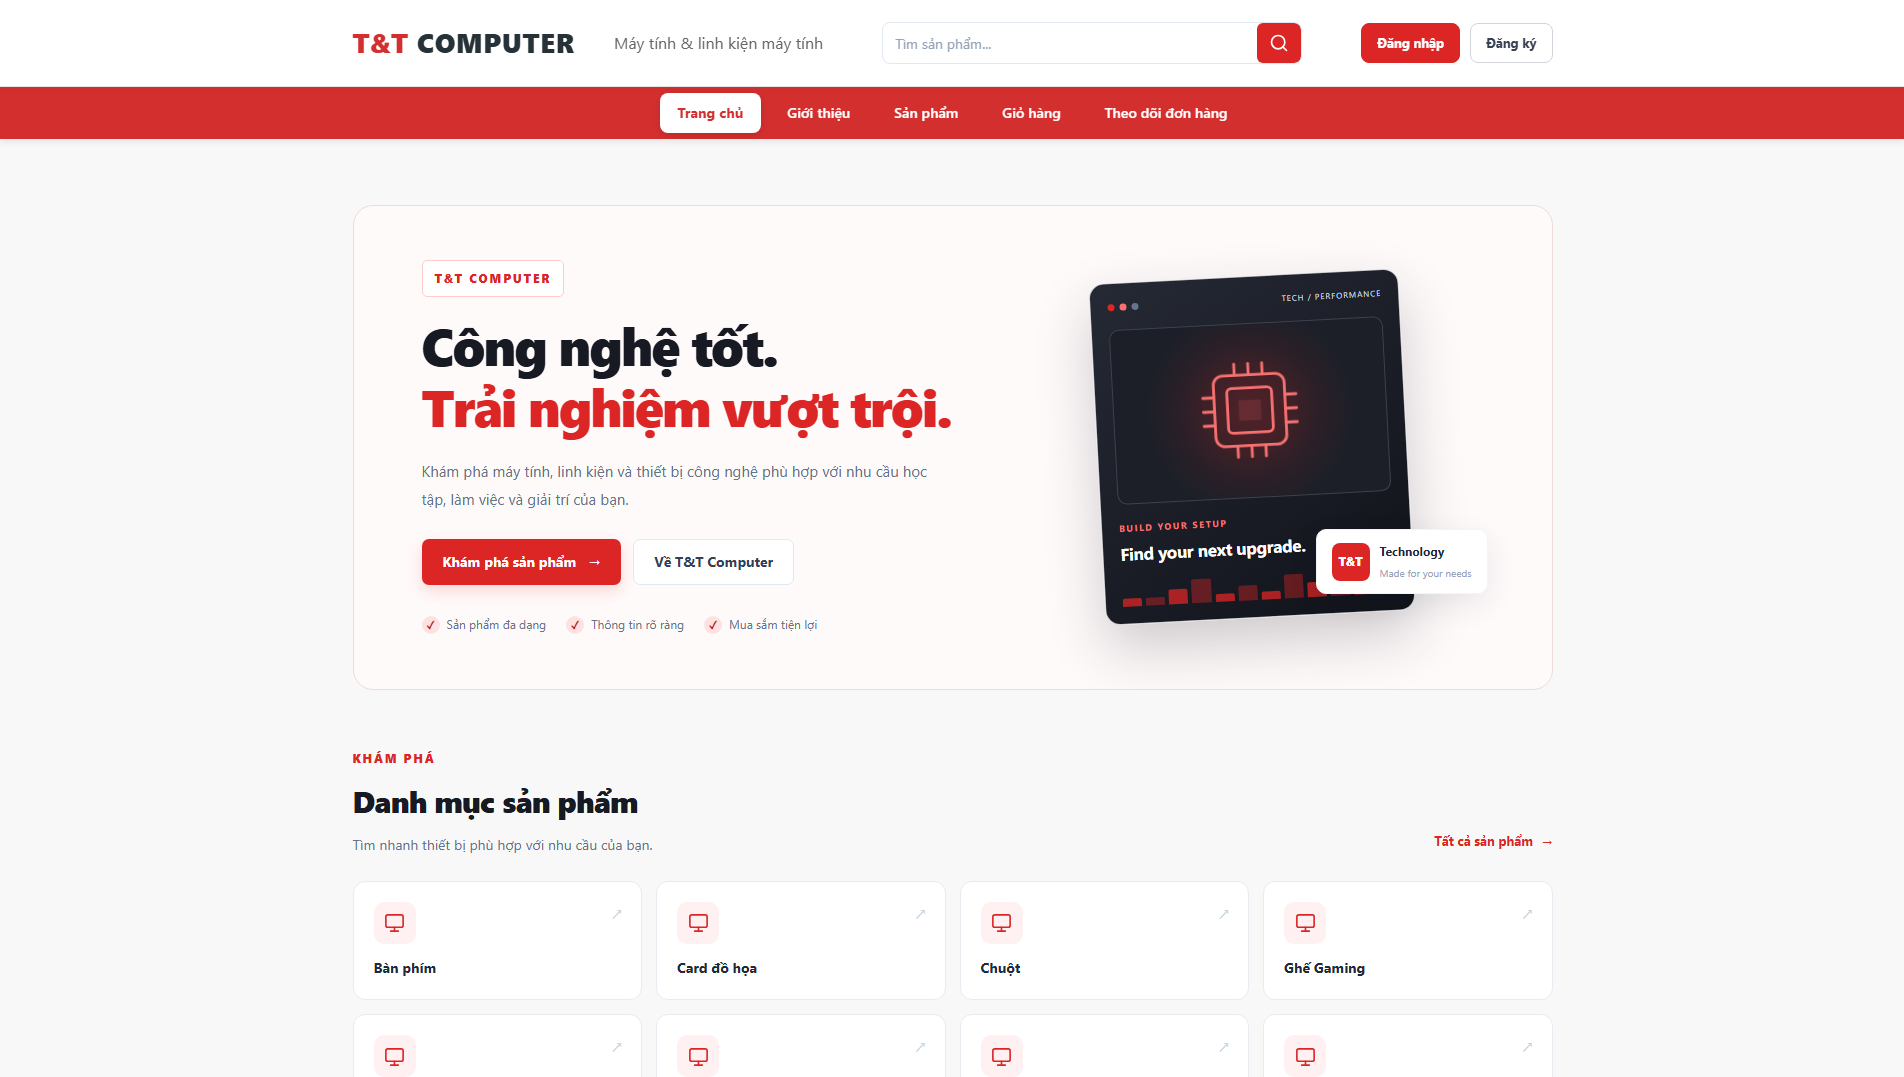
\includegraphics[width=0.95\textwidth,height=0.72\textheight,keepaspectratio]{TaiLieu/AnhChuong3/IMG01_trang_chu.png}
    \caption{Giao diện trang chủ T\&T Computer}
    \label{fig:img01-trang-chu}
\end{figure}

\section{Kết quả triển khai chức năng}
\subsection{Chức năng dành cho khách hàng}
Mã nguồn có các luồng tạo tài khoản, đăng nhập, đăng nhập hoặc liên kết Google, cập nhật hồ sơ và địa chỉ nhận hàng. Danh mục hỗ trợ tìm theo từ khóa, lọc theo danh mục, loại sản phẩm, thương hiệu và khoảng giá, sắp xếp theo tên hoặc giá, xem chi tiết sản phẩm. Bộ lọc không truy vấn các trường thông số kỹ thuật. Khách đã đăng nhập có thể quản lý giỏ hàng, áp dụng khuyến mãi/voucher và tạo đơn; máy chủ kiểm tra lại giá, ưu đãi và tồn kho trong quá trình đặt hàng.

Đơn COD được tạo ở trạng thái \textbf{Chưa thanh toán}; mã nguồn chưa có thao tác xác nhận đã thu tiền COD. Với thanh toán trực tuyến, mã nguồn khởi tạo checkout SePay Sandbox và xác minh IPN trước khi ghi giao dịch, cập nhật trạng thái đơn. SePay Sandbox chưa phải tích hợp production. Khách hàng có thể xem và hủy đơn khi còn ở trạng thái cho phép; không tìm thấy tác vụ nền tự động hủy đơn khi thanh toán lỗi hoặc quá hạn.

\begin{figure}[H]
    \centering
    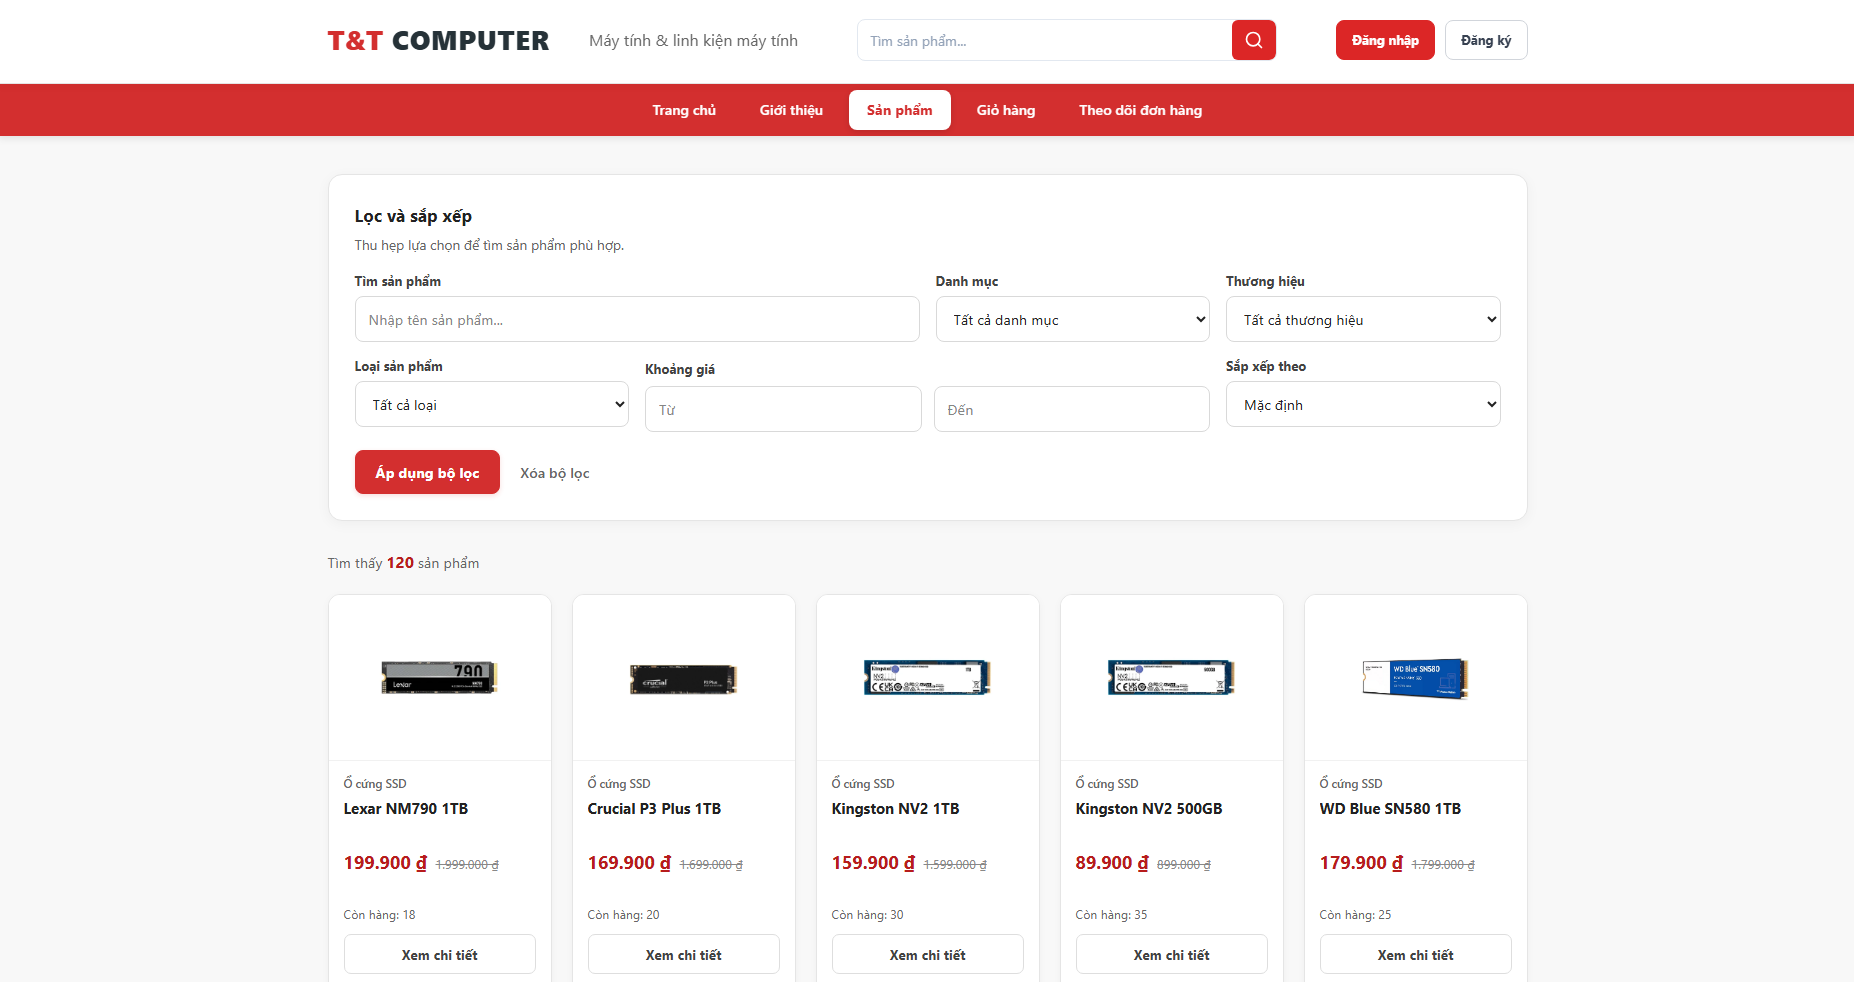
\includegraphics[width=0.95\textwidth,height=0.72\textheight,keepaspectratio]{TaiLieu/AnhChuong3/IMG02_danh_sach_san_pham.png}
    \caption{Danh sách sản phẩm}
    \label{fig:img02-danh-sach-san-pham}
\end{figure}
\begin{figure}[H]
    \centering
    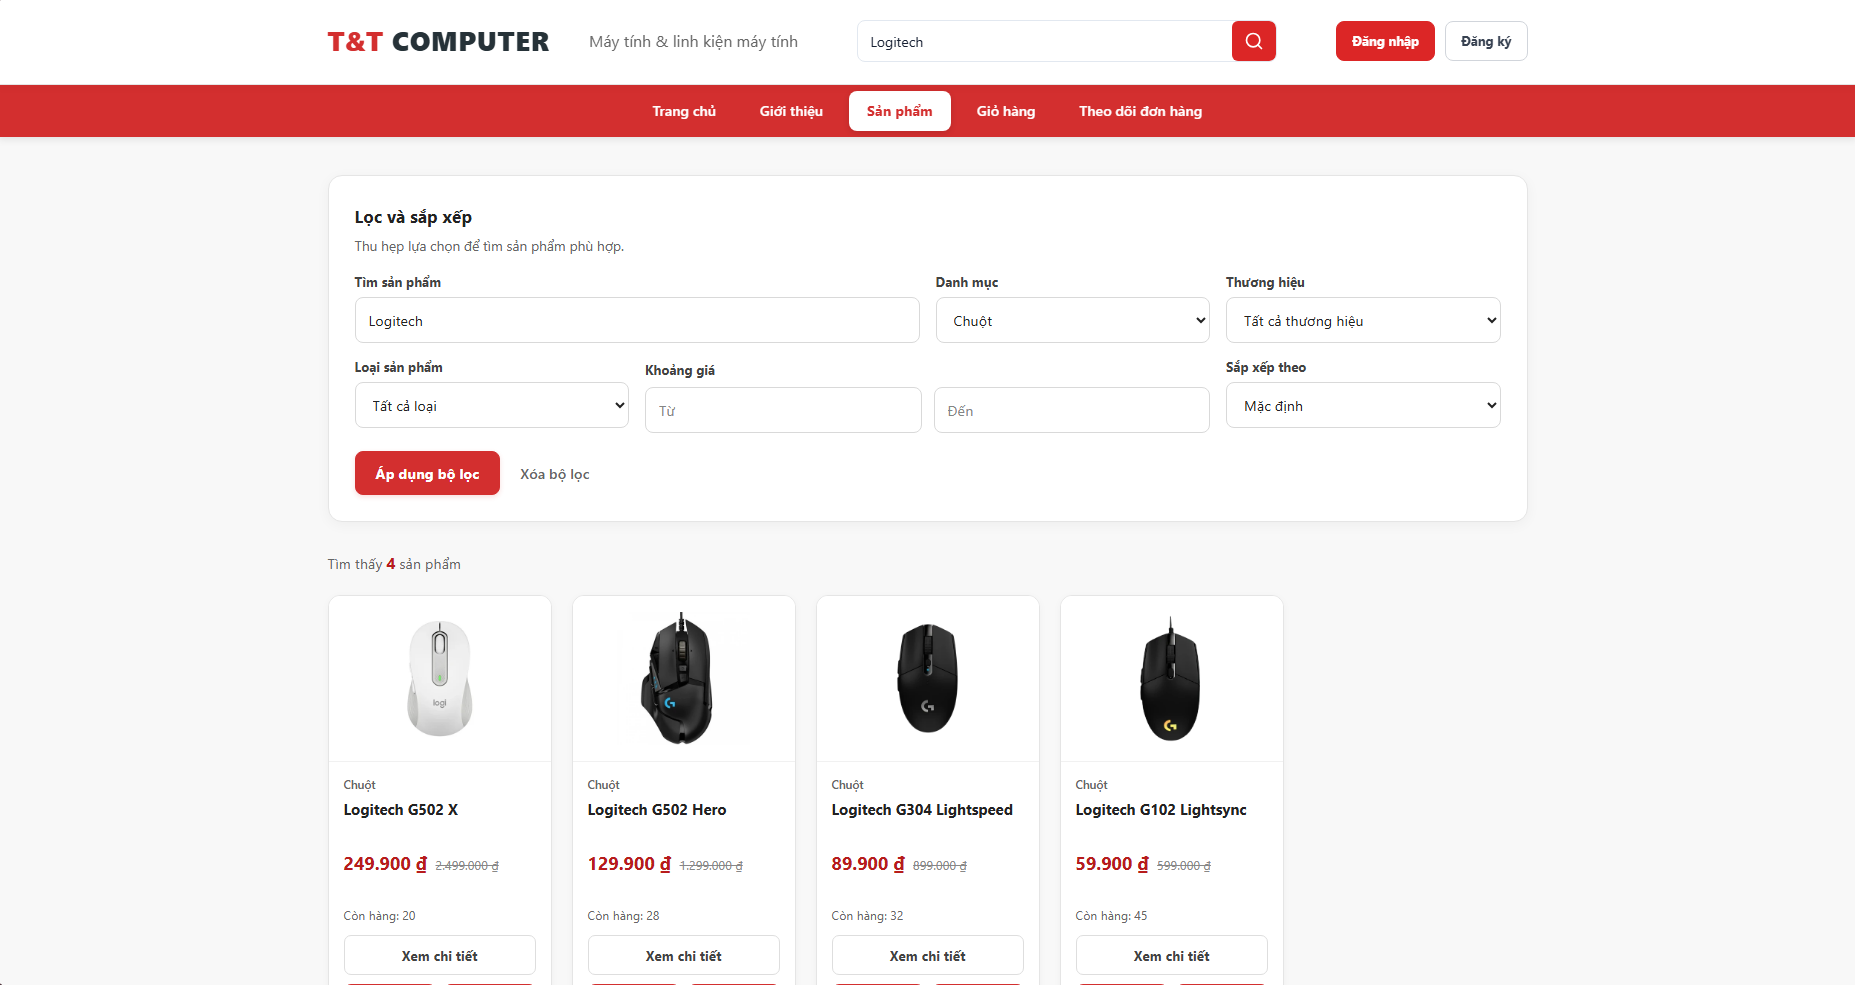
\includegraphics[width=0.95\textwidth,height=0.72\textheight,keepaspectratio]{TaiLieu/AnhChuong3/IMG03_tim_kiem_loc_san_pham.png}
    \caption{Tìm kiếm và lọc sản phẩm theo các tiêu chí hệ thống hỗ trợ}
    \label{fig:img03-tim-kiem-loc}
\end{figure}
\begin{figure}[H]
    \centering
    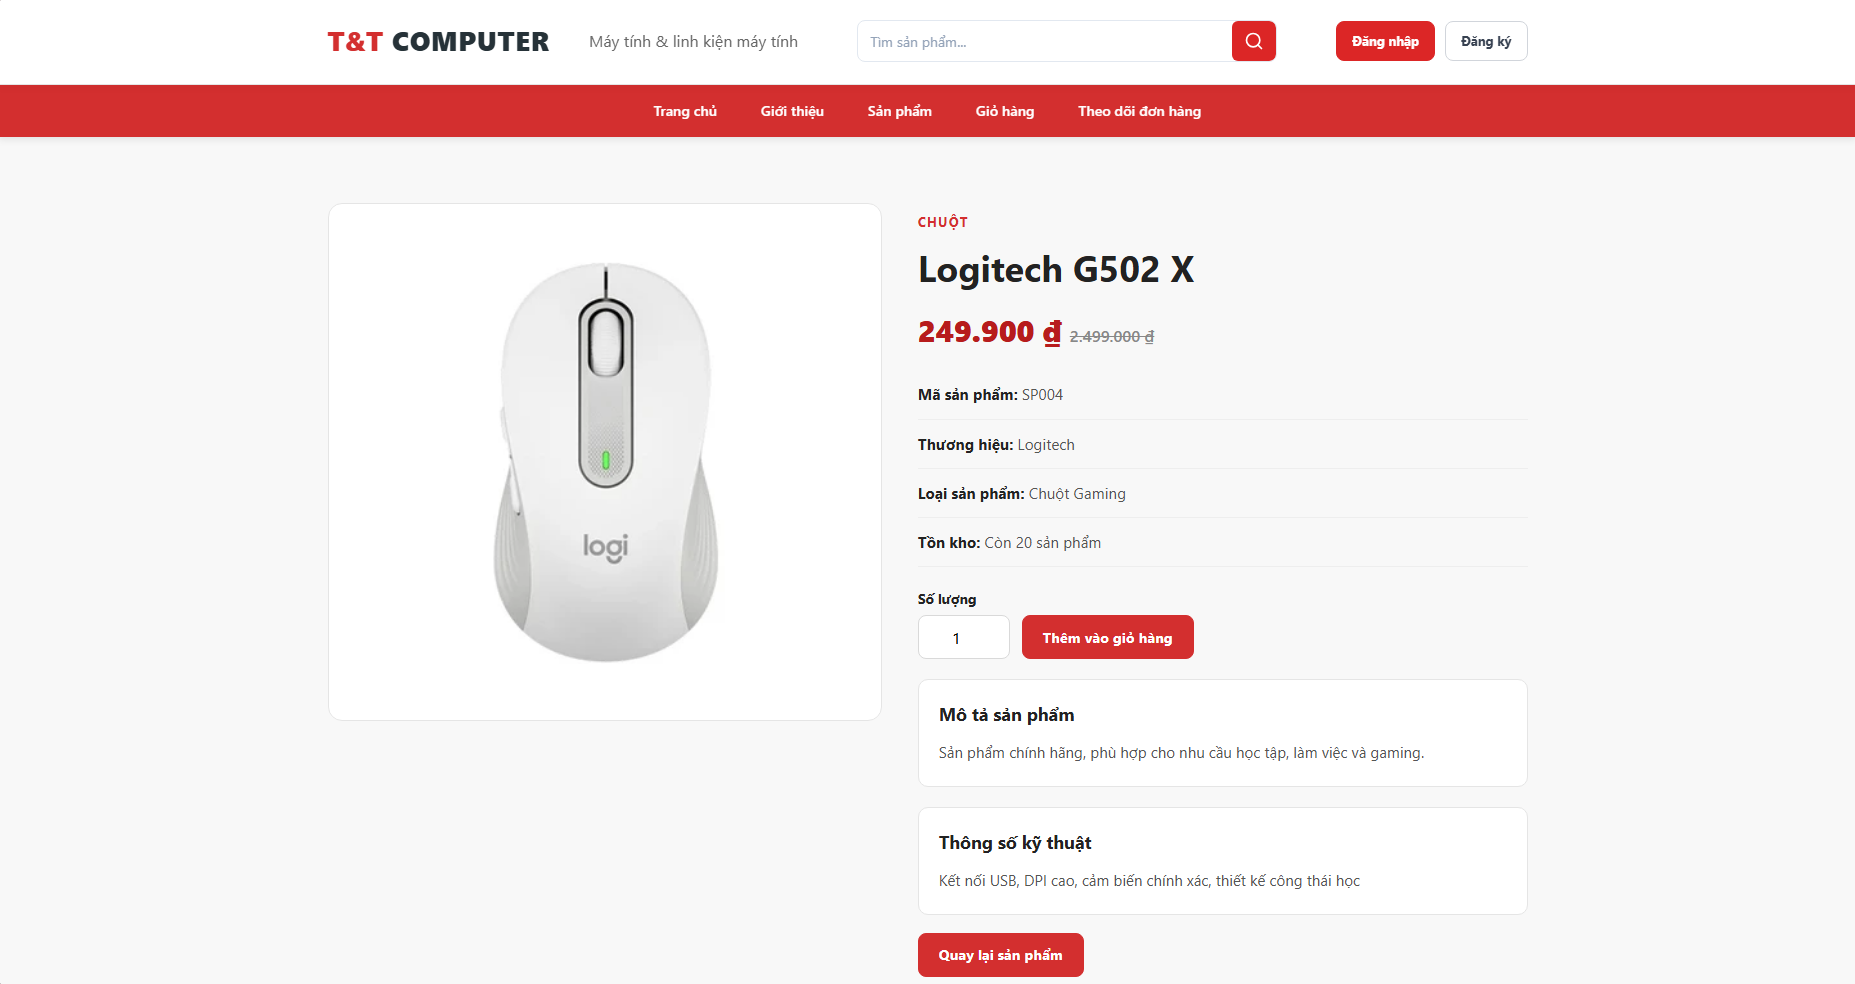
\includegraphics[width=0.95\textwidth,height=0.72\textheight,keepaspectratio]{TaiLieu/AnhChuong3/IMG04_chi_tiet_san_pham.png}
    \caption{Trang chi tiết sản phẩm}
    \label{fig:img04-chi-tiet-san-pham}
\end{figure}
\begin{figure}[H]
    \centering
    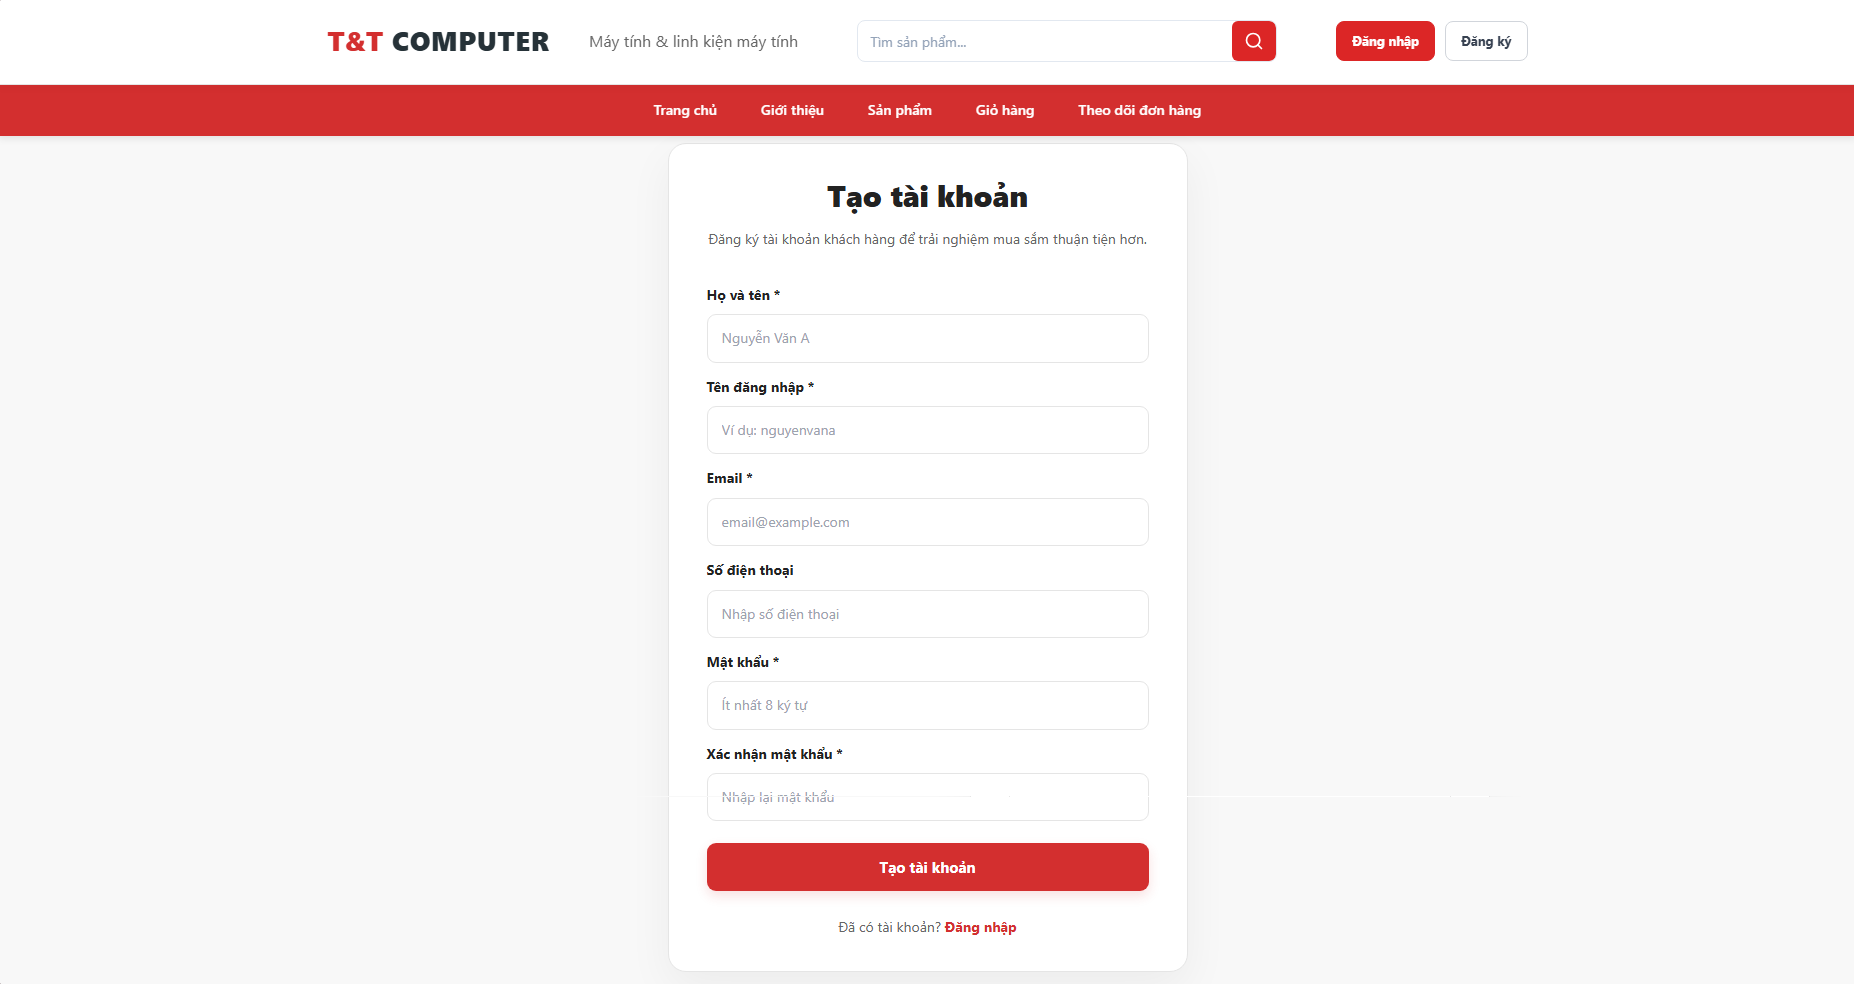
\includegraphics[width=0.85\textwidth,height=0.72\textheight,keepaspectratio]{TaiLieu/AnhChuong3/IMG05_dang_ky_tai_khoan.png}
    \caption{Giao diện đăng ký tài khoản}
    \label{fig:img05-dang-ky}
\end{figure}
\begin{figure}[H]
    \centering
    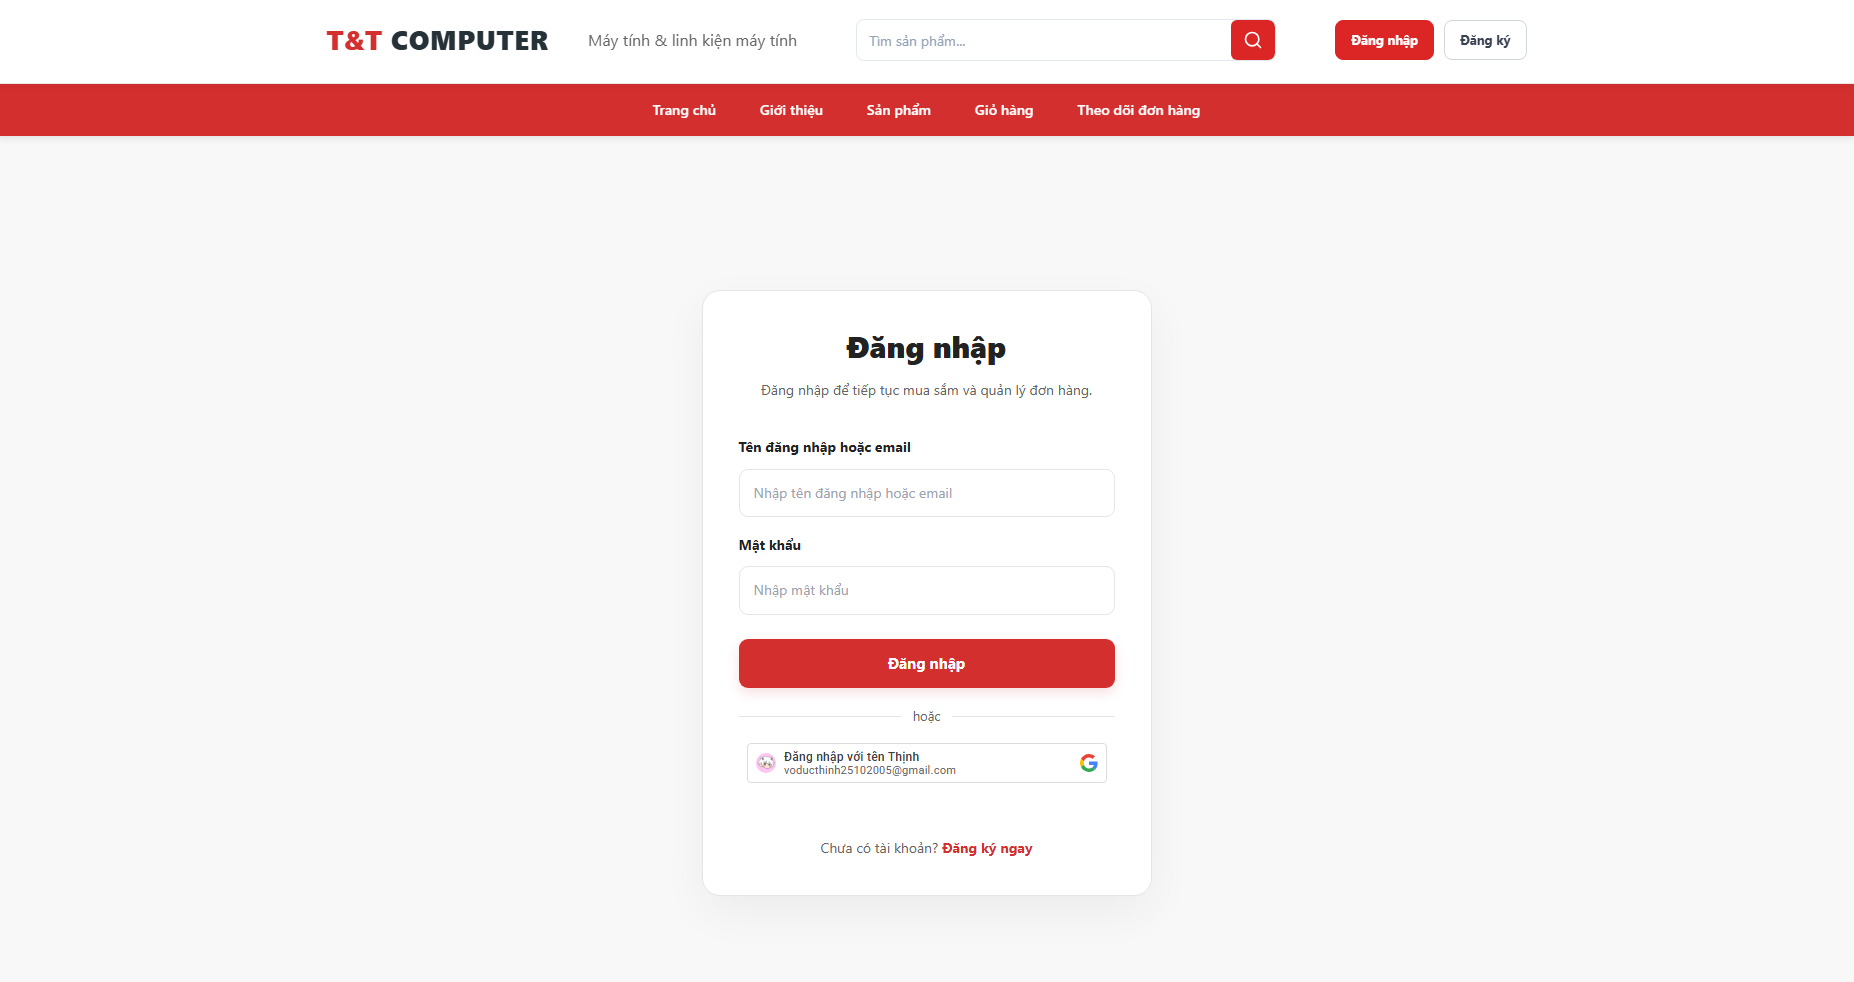
\includegraphics[width=0.85\textwidth,height=0.72\textheight,keepaspectratio]{TaiLieu/AnhChuong3/IMG06_dang_nhap.png}
    \caption{Giao diện đăng nhập}
    \label{fig:img06-dang-nhap}
\end{figure}
\begin{figure}[H]
    \centering
    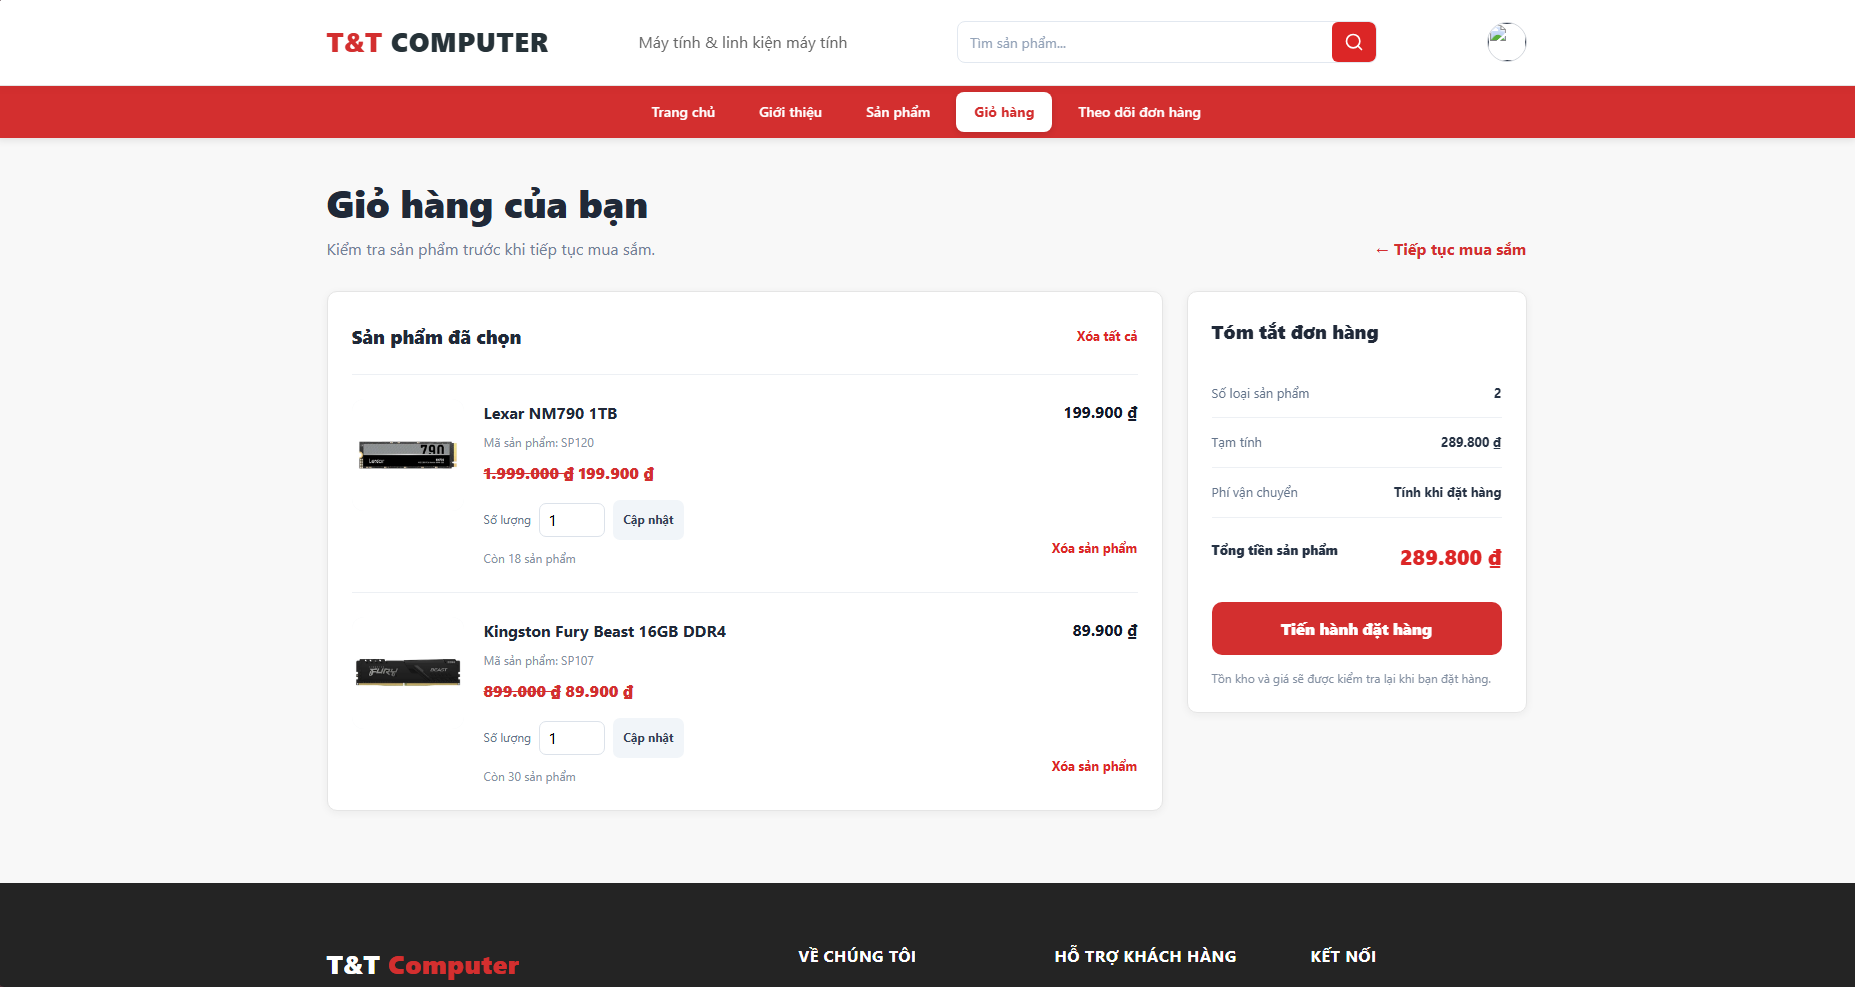
\includegraphics[width=0.95\textwidth,height=0.72\textheight,keepaspectratio]{TaiLieu/AnhChuong3/IMG07_gio_hang.png}
    \caption{Giỏ hàng khách hàng}
    \label{fig:img07-gio-hang}
\end{figure}
\begin{figure}[H]
    \centering
    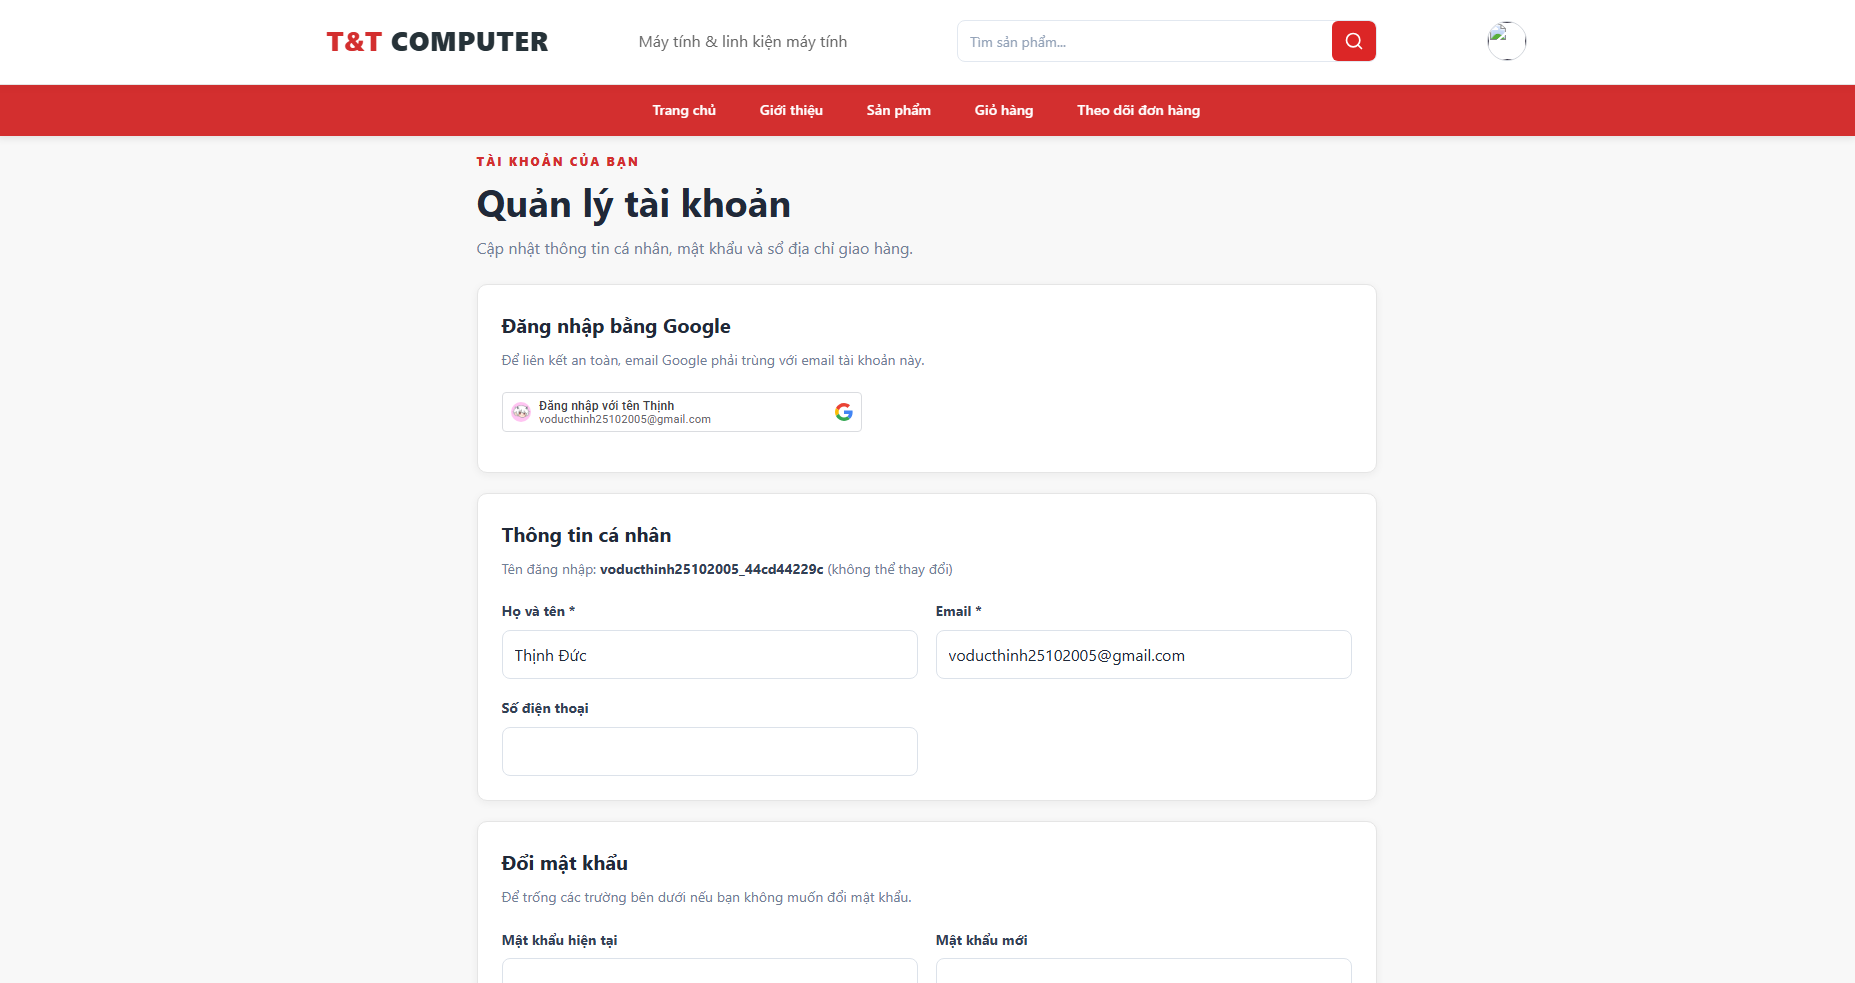
\includegraphics[width=0.95\textwidth,height=0.72\textheight,keepaspectratio]{TaiLieu/AnhChuong3/IMG08_thong_tin_tai_khoan.png}
    \caption{Thông tin tài khoản khách hàng}
    \label{fig:img08-tai-khoan}
\end{figure}

\subsection{Chức năng dành cho nhân viên}
Theo các kiểm tra quyền trong controller, nhân viên được tham gia xử lý trạng thái đơn hàng và tra cứu tồn kho trong phạm vi quyền được cấp. Nhân viên không có quyền điều chỉnh số lượng kho qua chức năng quản lý kho dành cho quản trị viên. Việc hoàn tồn trong một số quy trình đơn hàng được thực hiện bởi nghiệp vụ xử lý đơn, có ghi lịch sử kho; quyền nhập hoặc điều chỉnh kho độc lập thuộc vai trò quản trị viên.

\begin{figure}[H]
    \centering
    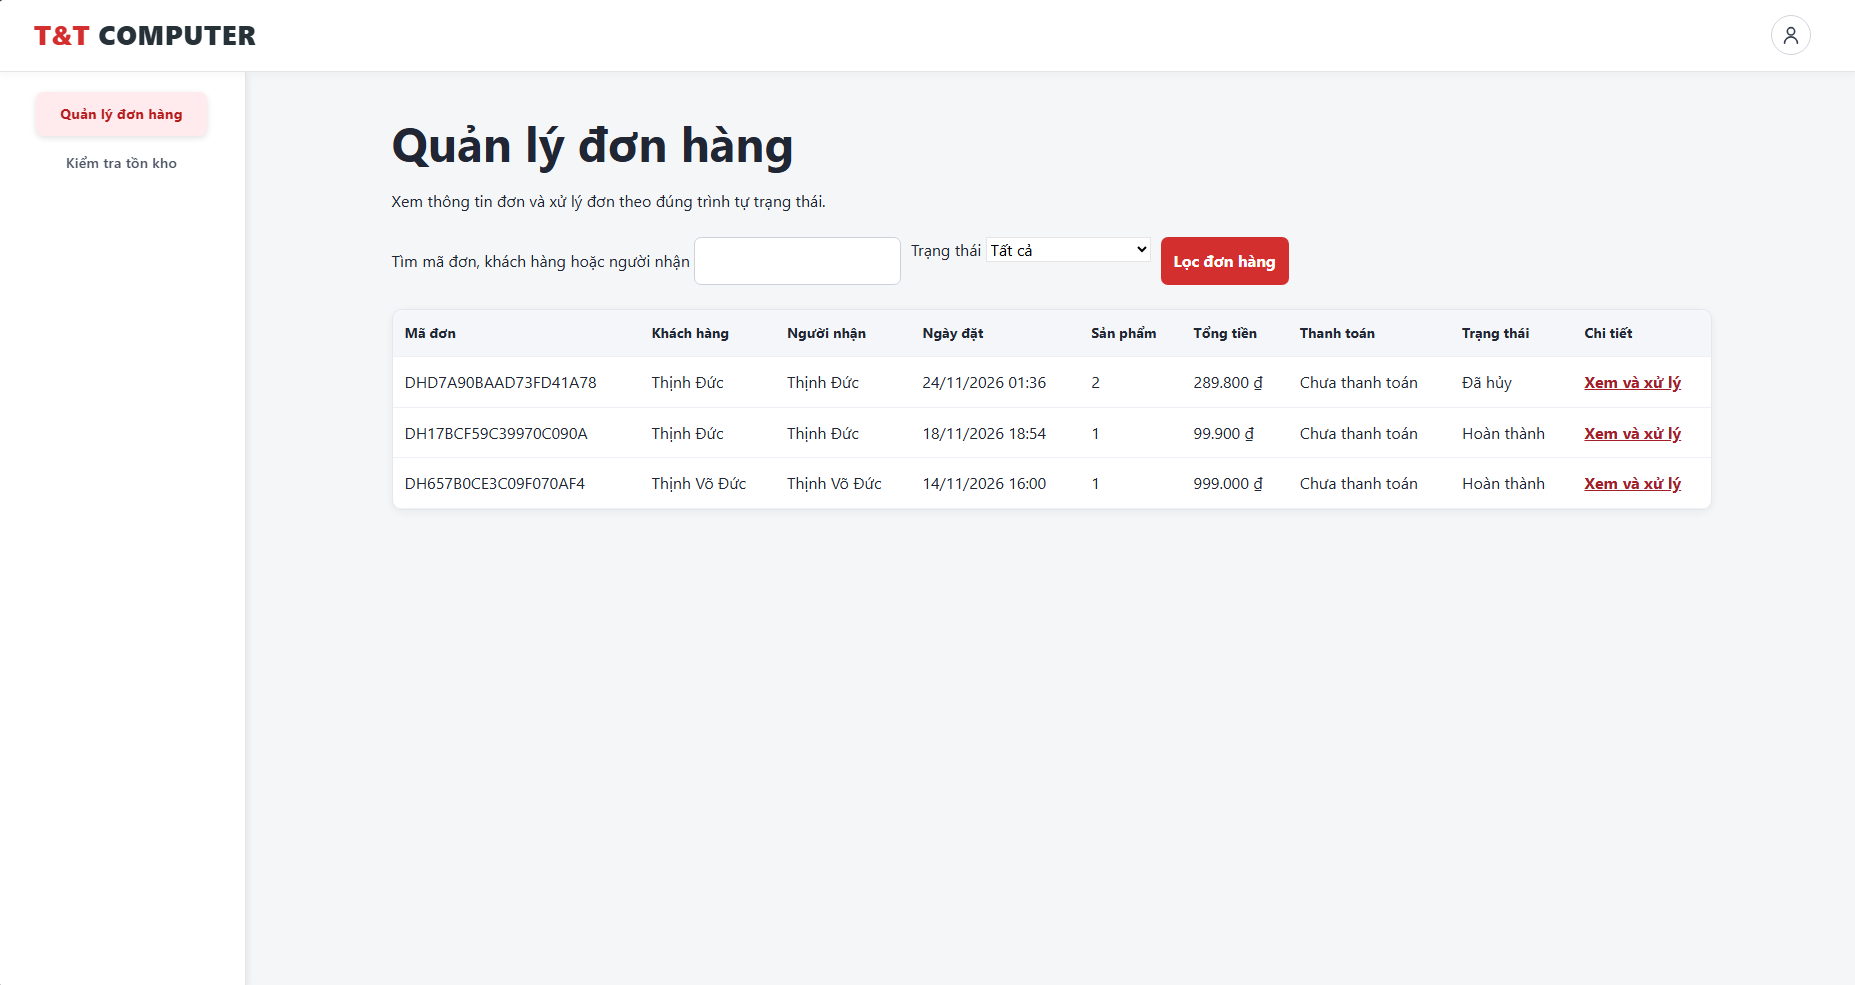
\includegraphics[width=0.95\textwidth,height=0.72\textheight,keepaspectratio]{TaiLieu/AnhChuong3/IMG16_nhan_vien_danh_sach_don.png}
    \caption{Danh sách đơn hàng trong giao diện nhân viên}
    \label{fig:img16-nv-danh-sach-don}
\end{figure}
\begin{figure}[H]
    \centering
    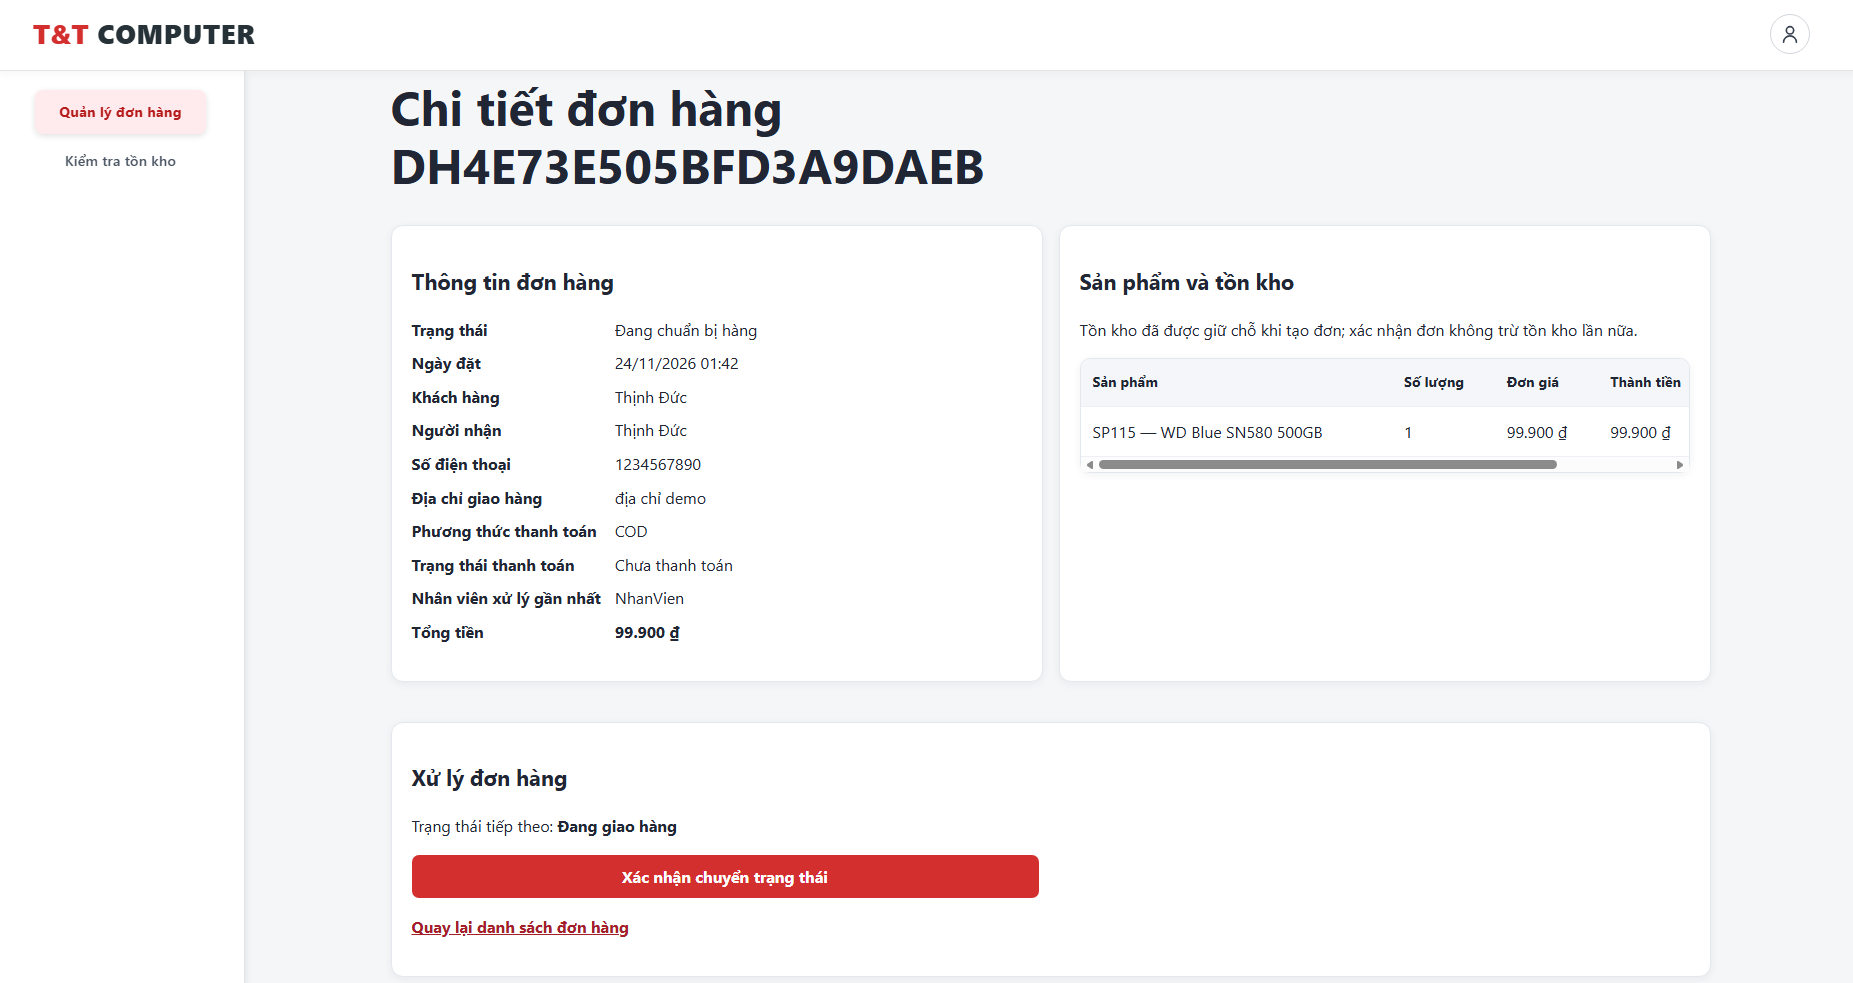
\includegraphics[width=0.95\textwidth,height=0.72\textheight,keepaspectratio]{TaiLieu/AnhChuong3/IMG17_nhan_vien_cap_nhat_trang_thai_don.png}
    \caption{Cập nhật trạng thái đơn hàng theo quyền nhân viên}
    \label{fig:img17-nv-cap-nhat-don}
\end{figure}
\begin{figure}[H]
    \centering
    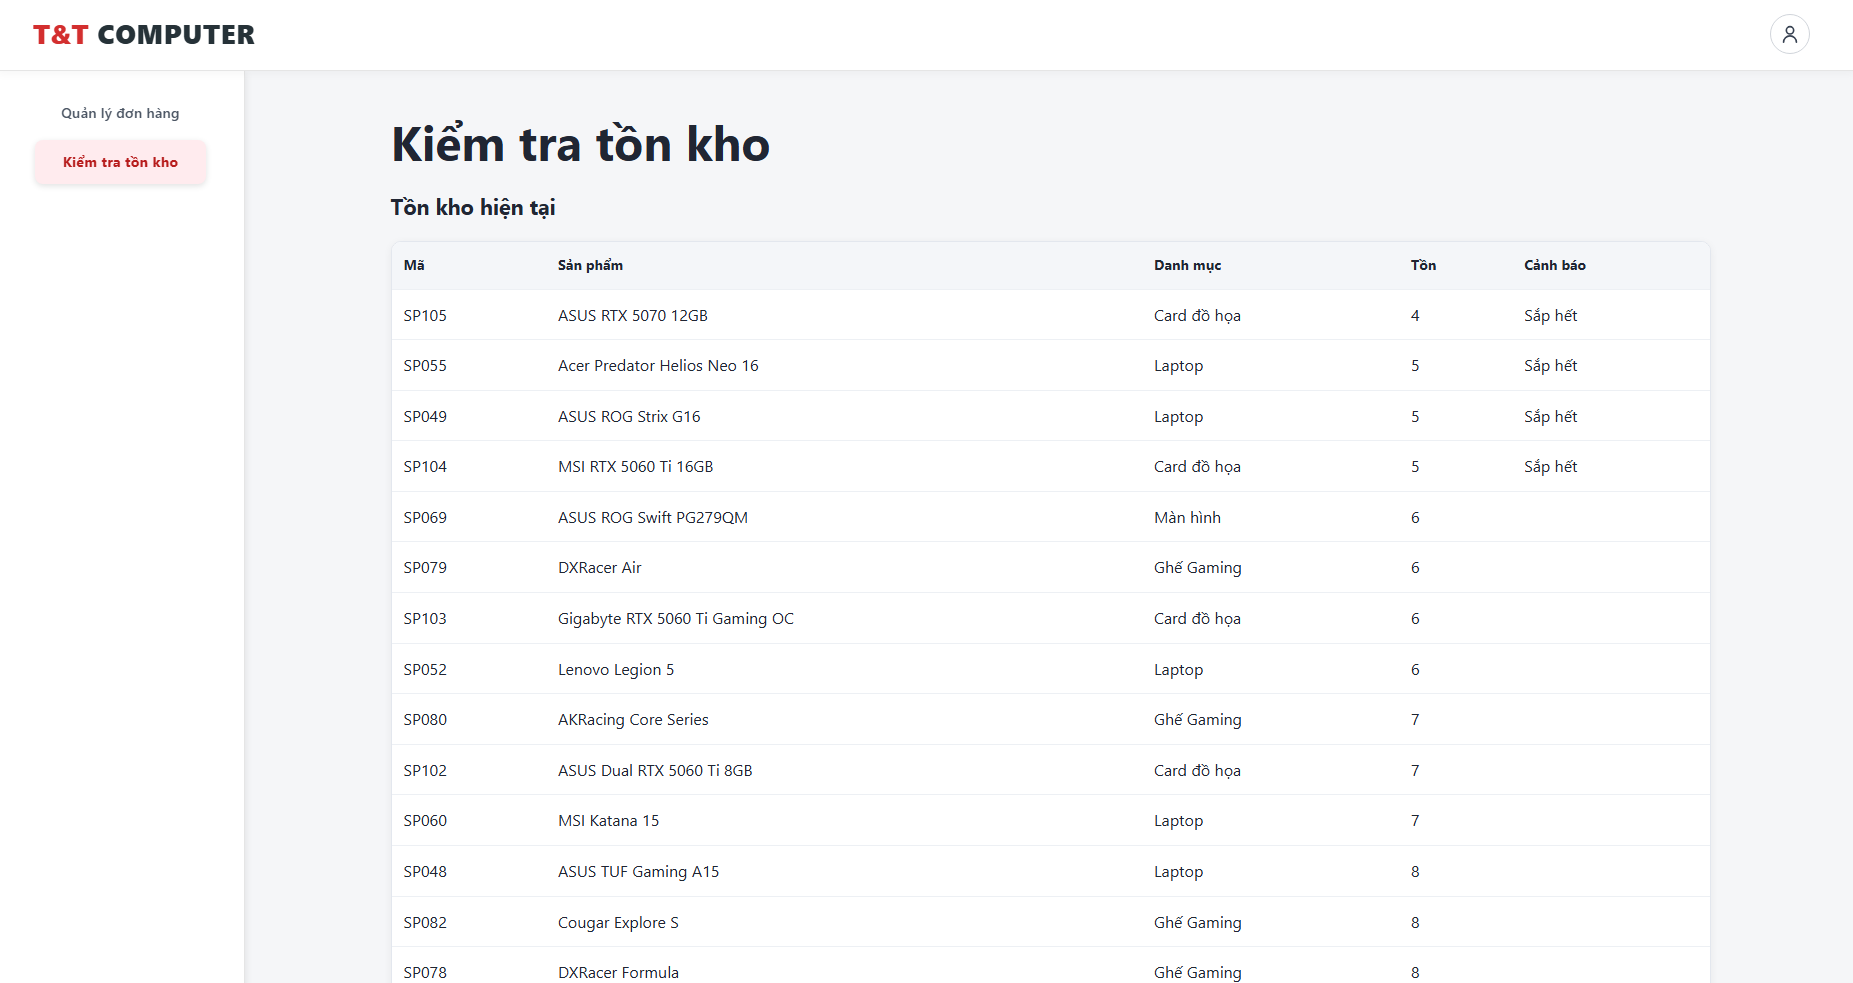
\includegraphics[width=0.95\textwidth,height=0.72\textheight,keepaspectratio]{TaiLieu/AnhChuong3/IMG18_nhan_vien_xem_ton_kho.png}
    \caption{Tra cứu tồn kho trong giao diện nhân viên}
    \label{fig:img18-nv-ton-kho}
\end{figure}

\subsection{Chức năng dành cho quản trị viên}
Các màn hình quản trị và controller hiện có hỗ trợ quản lý sản phẩm, danh mục, tài khoản, đơn hàng, tồn kho, chương trình giảm giá, voucher và thống kê. Quản lý kho có thao tác nhập/điều chỉnh và lưu lịch sử; thống kê thể hiện tình hình đơn, doanh thu và sản phẩm/tồn kho theo chức năng trong mã nguồn. Không có dữ liệu giá vốn trong schema hiện tại để xác nhận báo cáo lợi nhuận.

\begin{figure}[H]
    \centering
    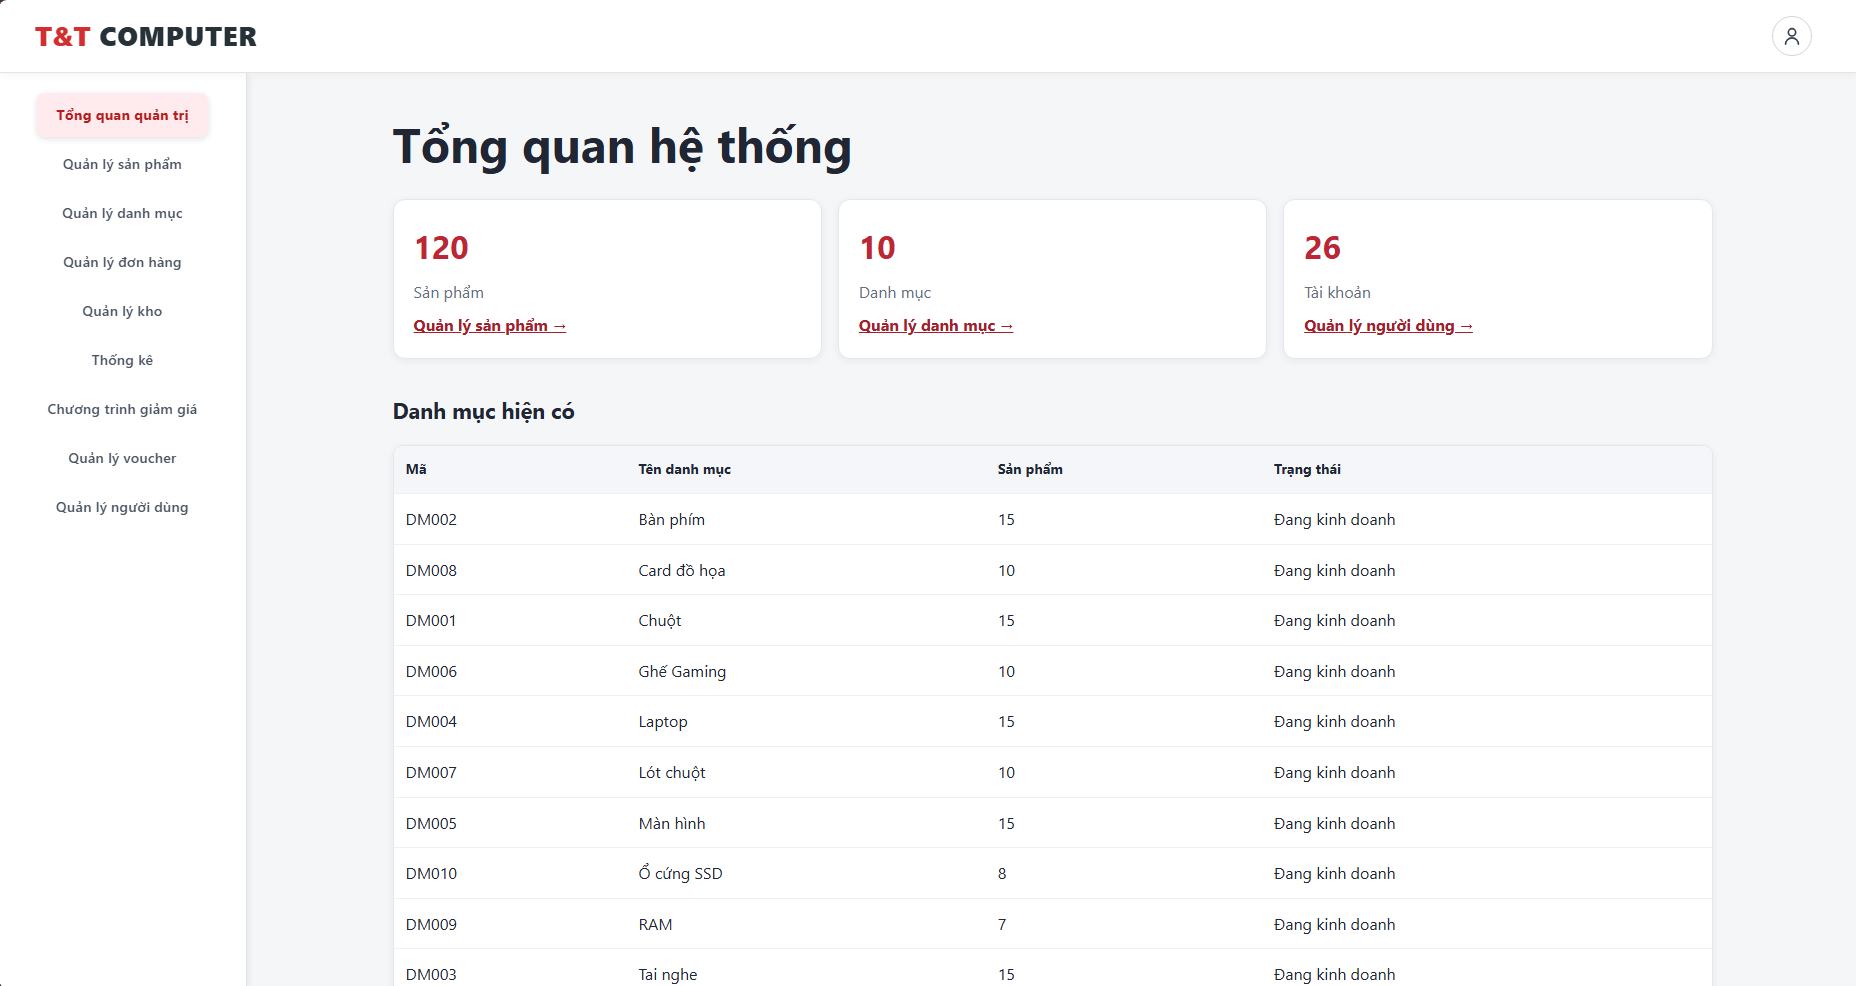
\includegraphics[width=0.95\textwidth,height=0.72\textheight,keepaspectratio]{TaiLieu/AnhChuong3/IMG19_admin_dashboard.png}
    \caption{Bảng điều khiển quản trị}
    \label{fig:img19-admin-dashboard}
\end{figure}
\begin{figure}[H]
    \centering
    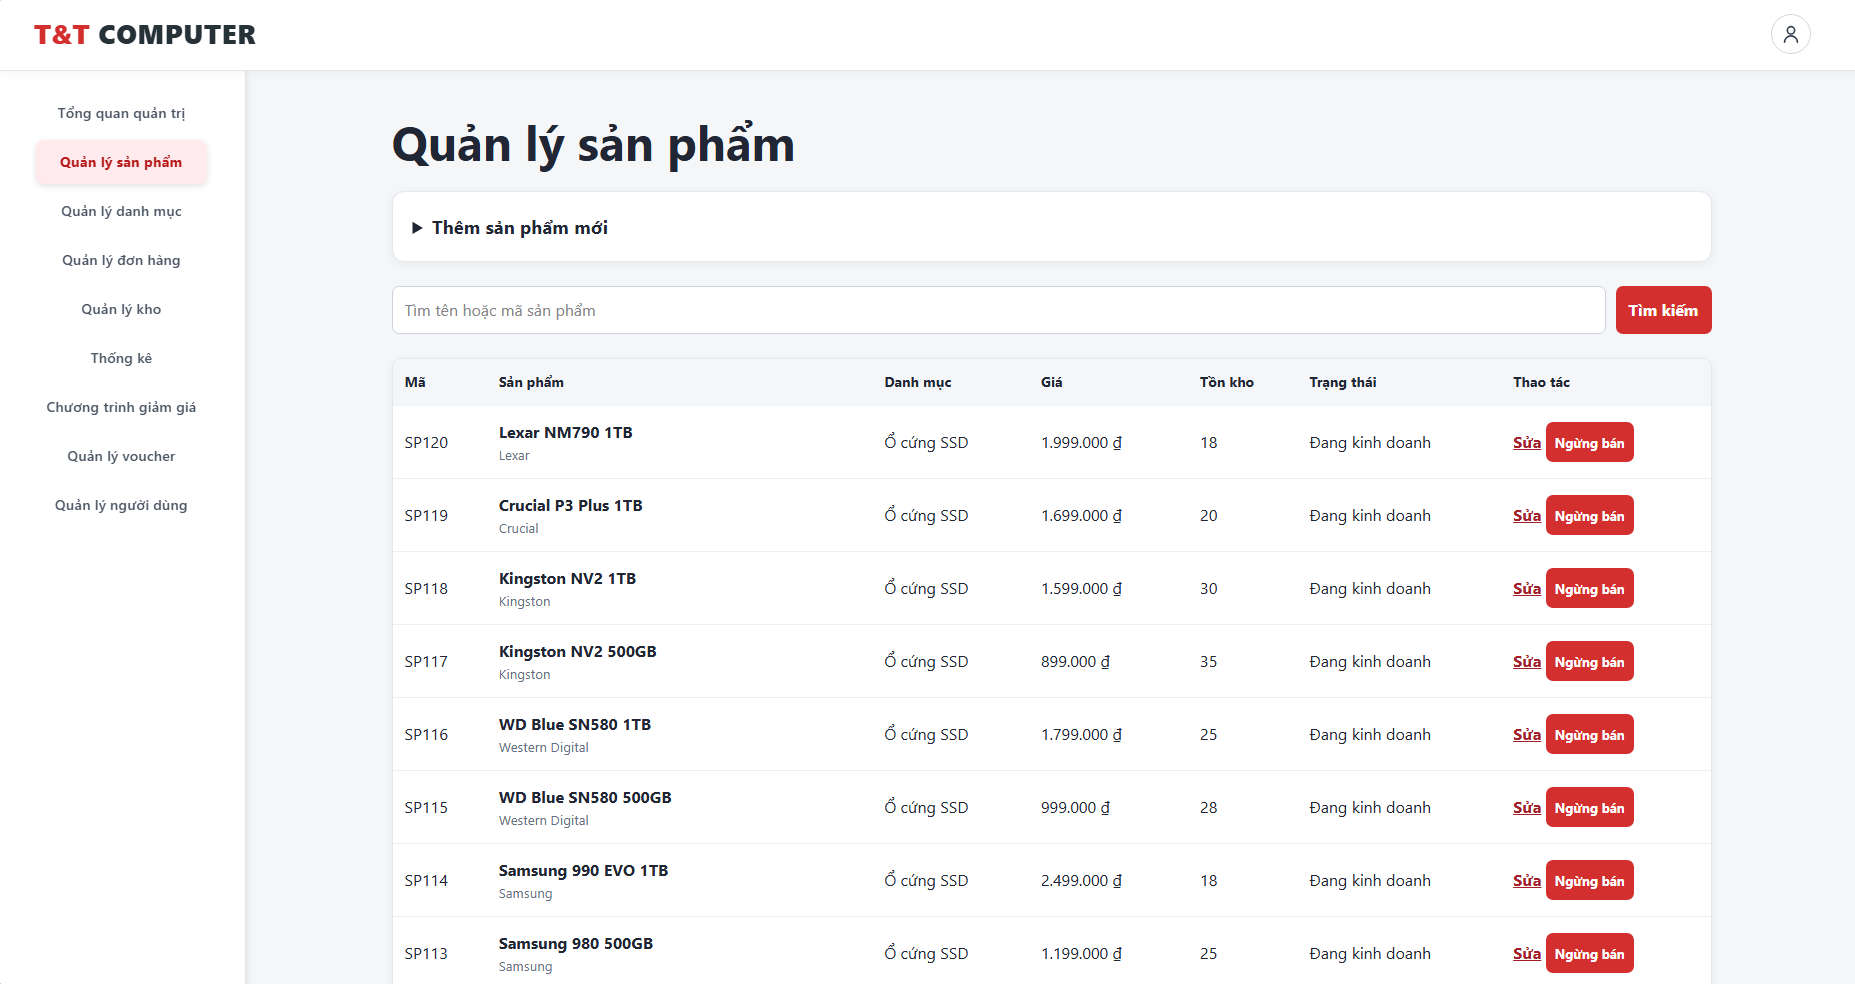
\includegraphics[width=0.95\textwidth,height=0.72\textheight,keepaspectratio]{TaiLieu/AnhChuong3/IMG20_admin_quan_ly_san_pham.png}
    \caption{Quản lý sản phẩm}
    \label{fig:img20-admin-san-pham}
\end{figure}
\begin{figure}[H]
    \centering
    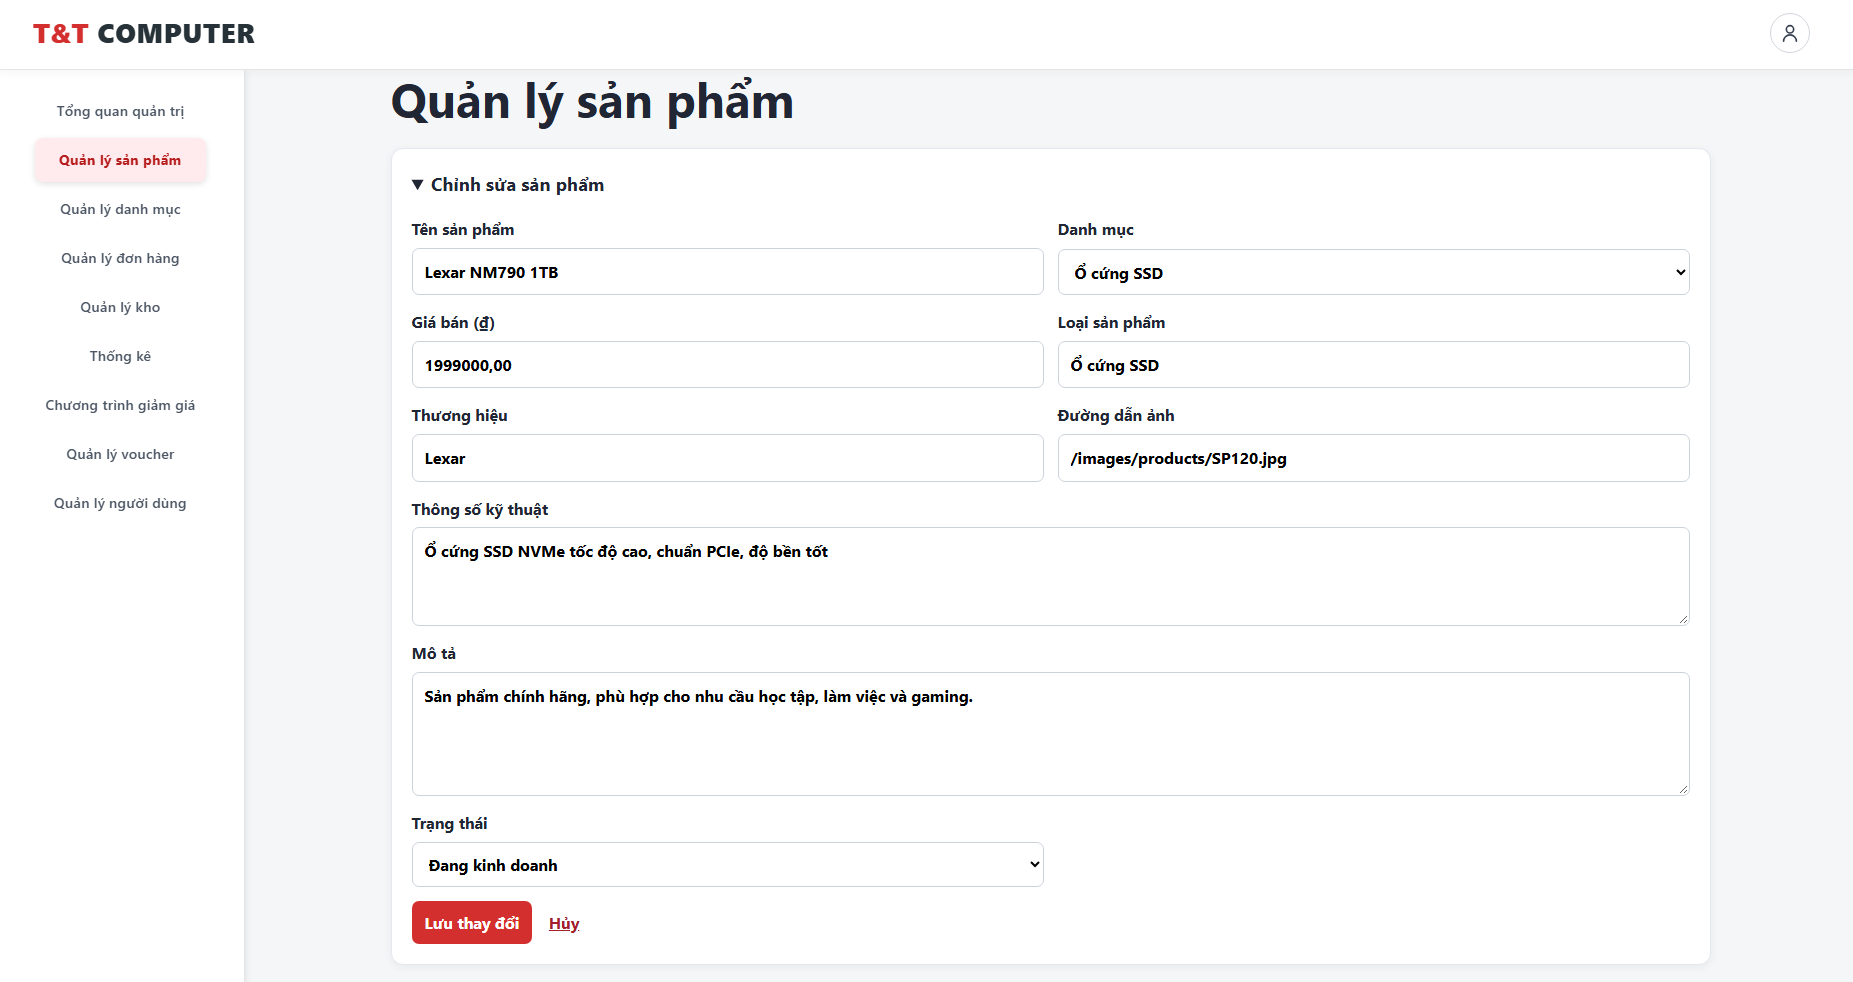
\includegraphics[width=0.95\textwidth,height=0.72\textheight,keepaspectratio]{TaiLieu/AnhChuong3/IMG21_admin_them_sua_san_pham.png}
    \caption{Biểu mẫu thêm hoặc cập nhật sản phẩm}
    \label{fig:img21-admin-form-san-pham}
\end{figure}
\begin{figure}[H]
    \centering
    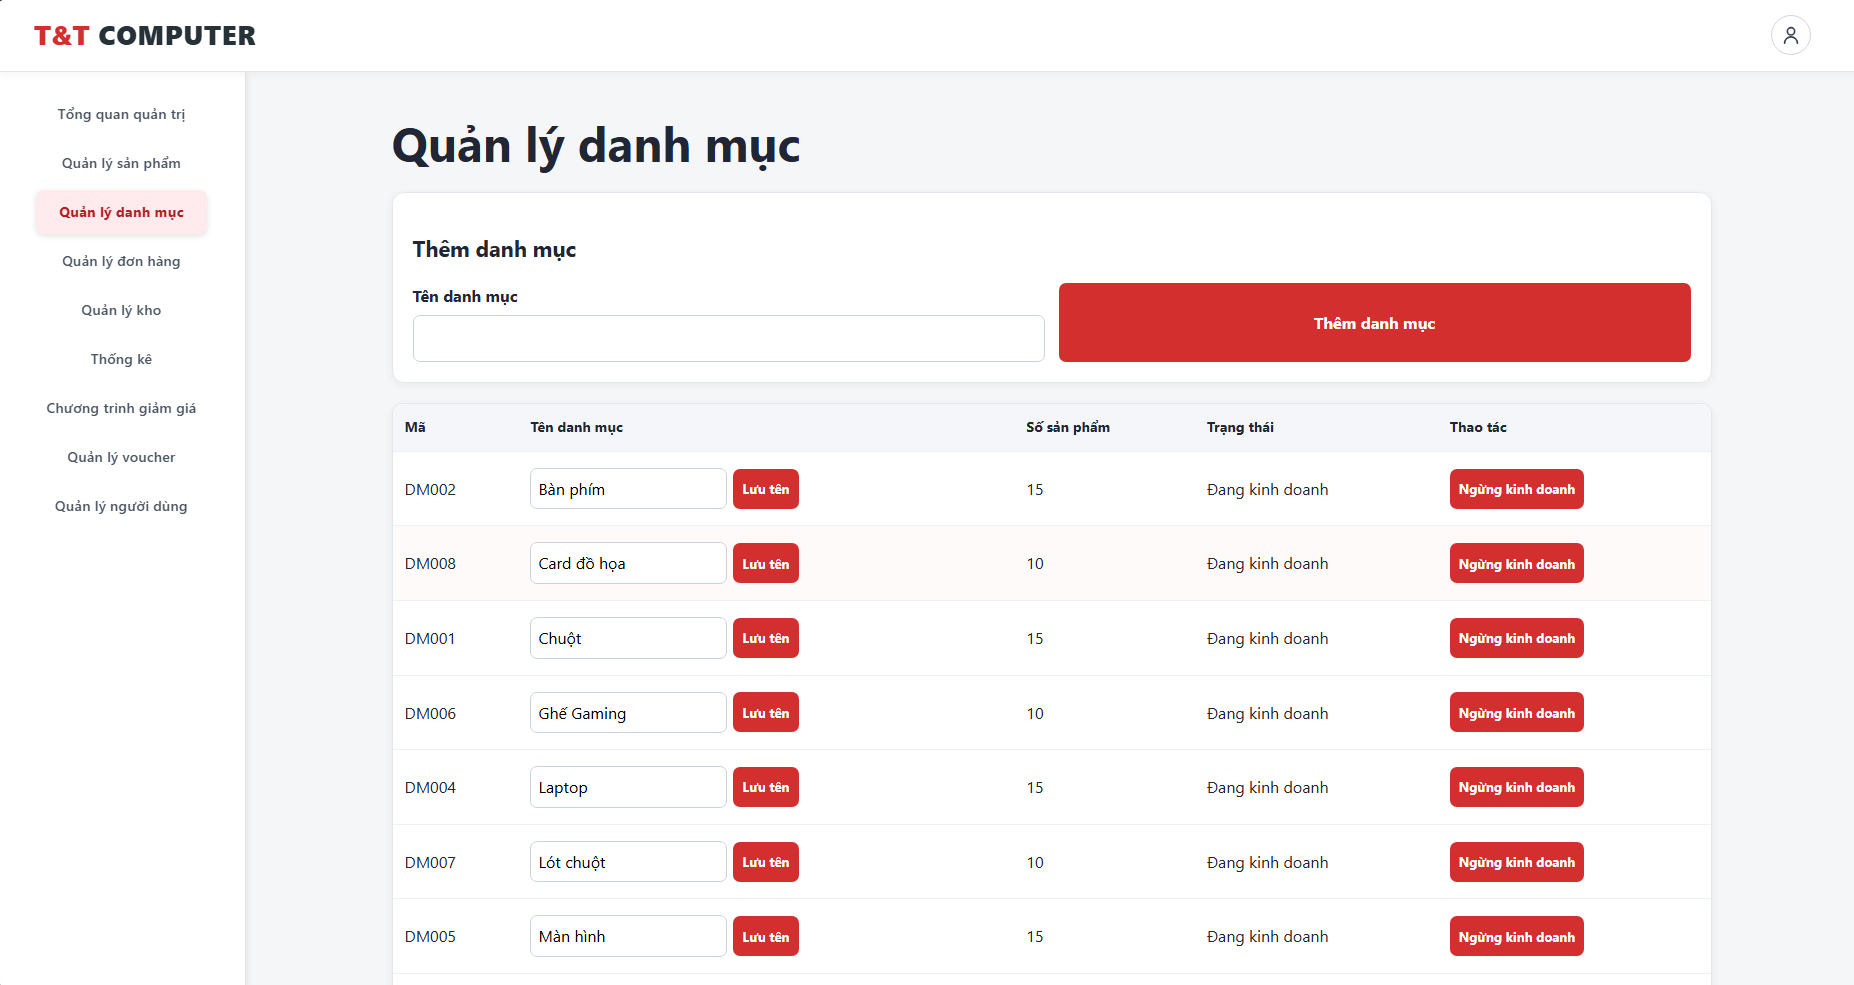
\includegraphics[width=0.95\textwidth,height=0.72\textheight,keepaspectratio]{TaiLieu/AnhChuong3/IMG22_admin_quan_ly_danh_muc.png}
    \caption{Quản lý danh mục sản phẩm}
    \label{fig:img22-admin-danh-muc}
\end{figure}
\begin{figure}[H]
    \centering
    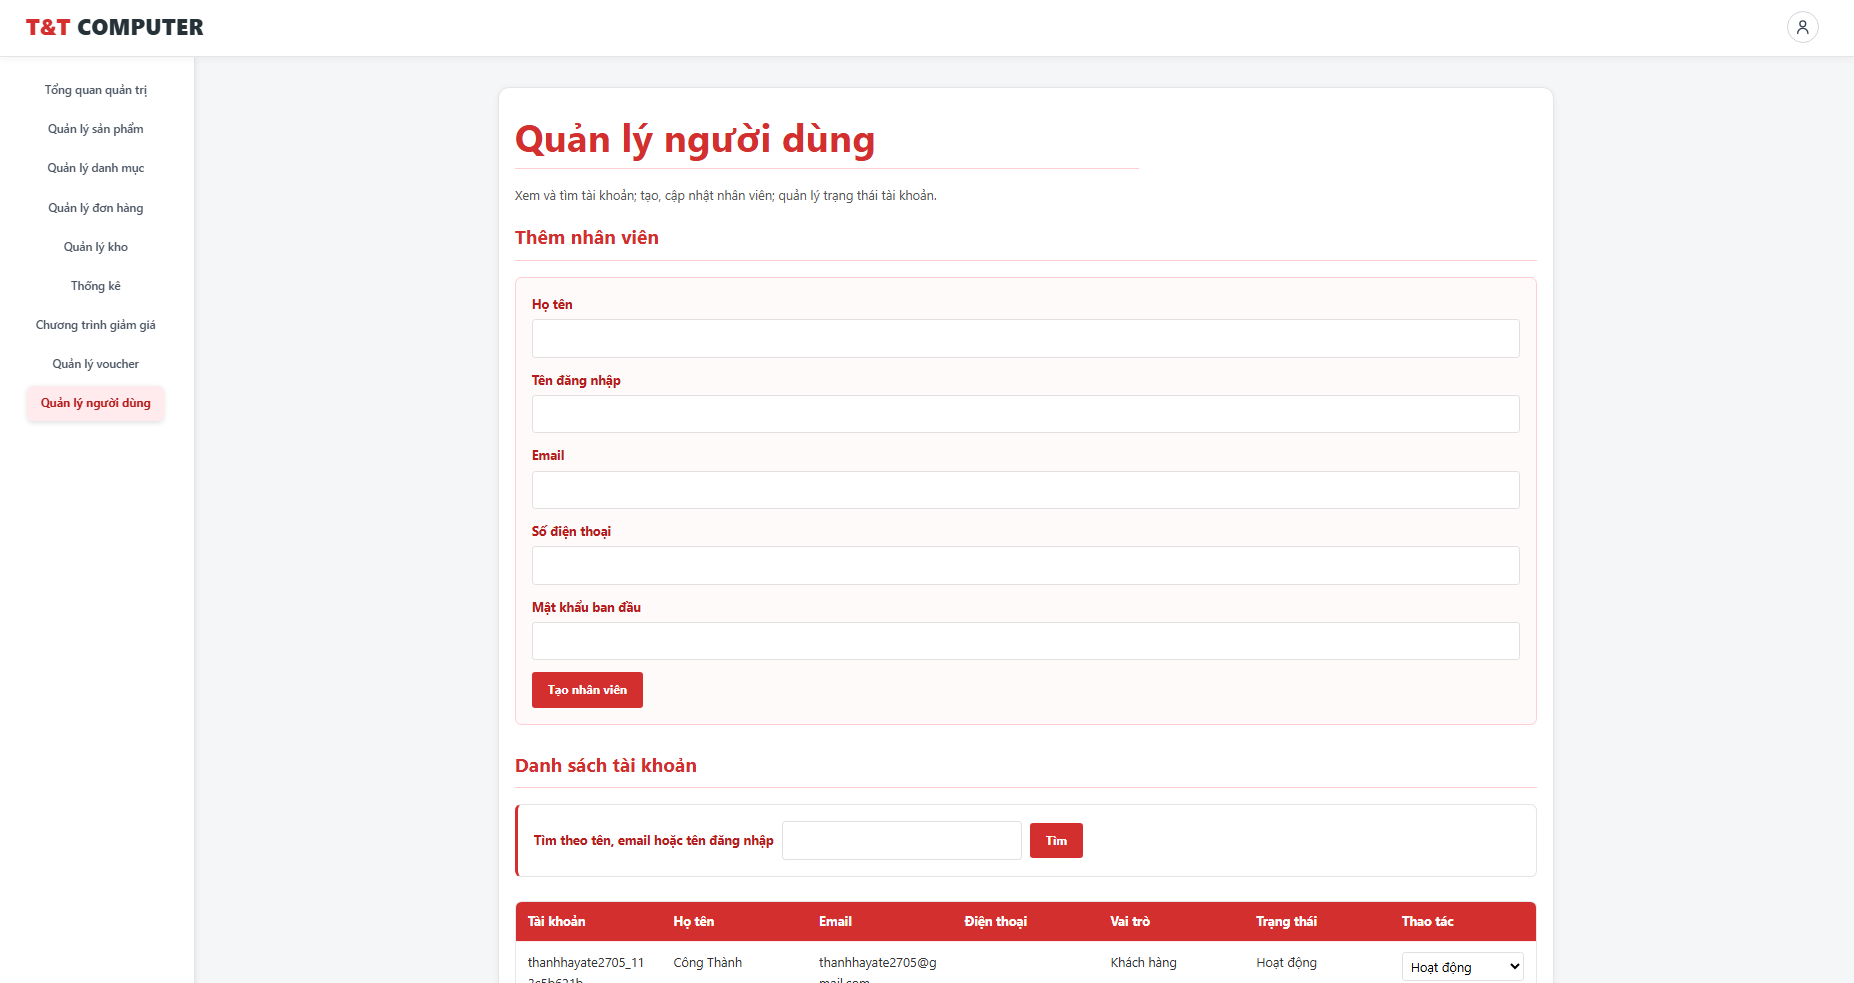
\includegraphics[width=0.95\textwidth,height=0.72\textheight,keepaspectratio]{TaiLieu/AnhChuong3/IMG23_admin_quan_ly_nguoi_dung.png}
    \caption{Quản lý tài khoản người dùng}
    \label{fig:img23-admin-nguoi-dung}
\end{figure}
\begin{figure}[H]
    \centering
    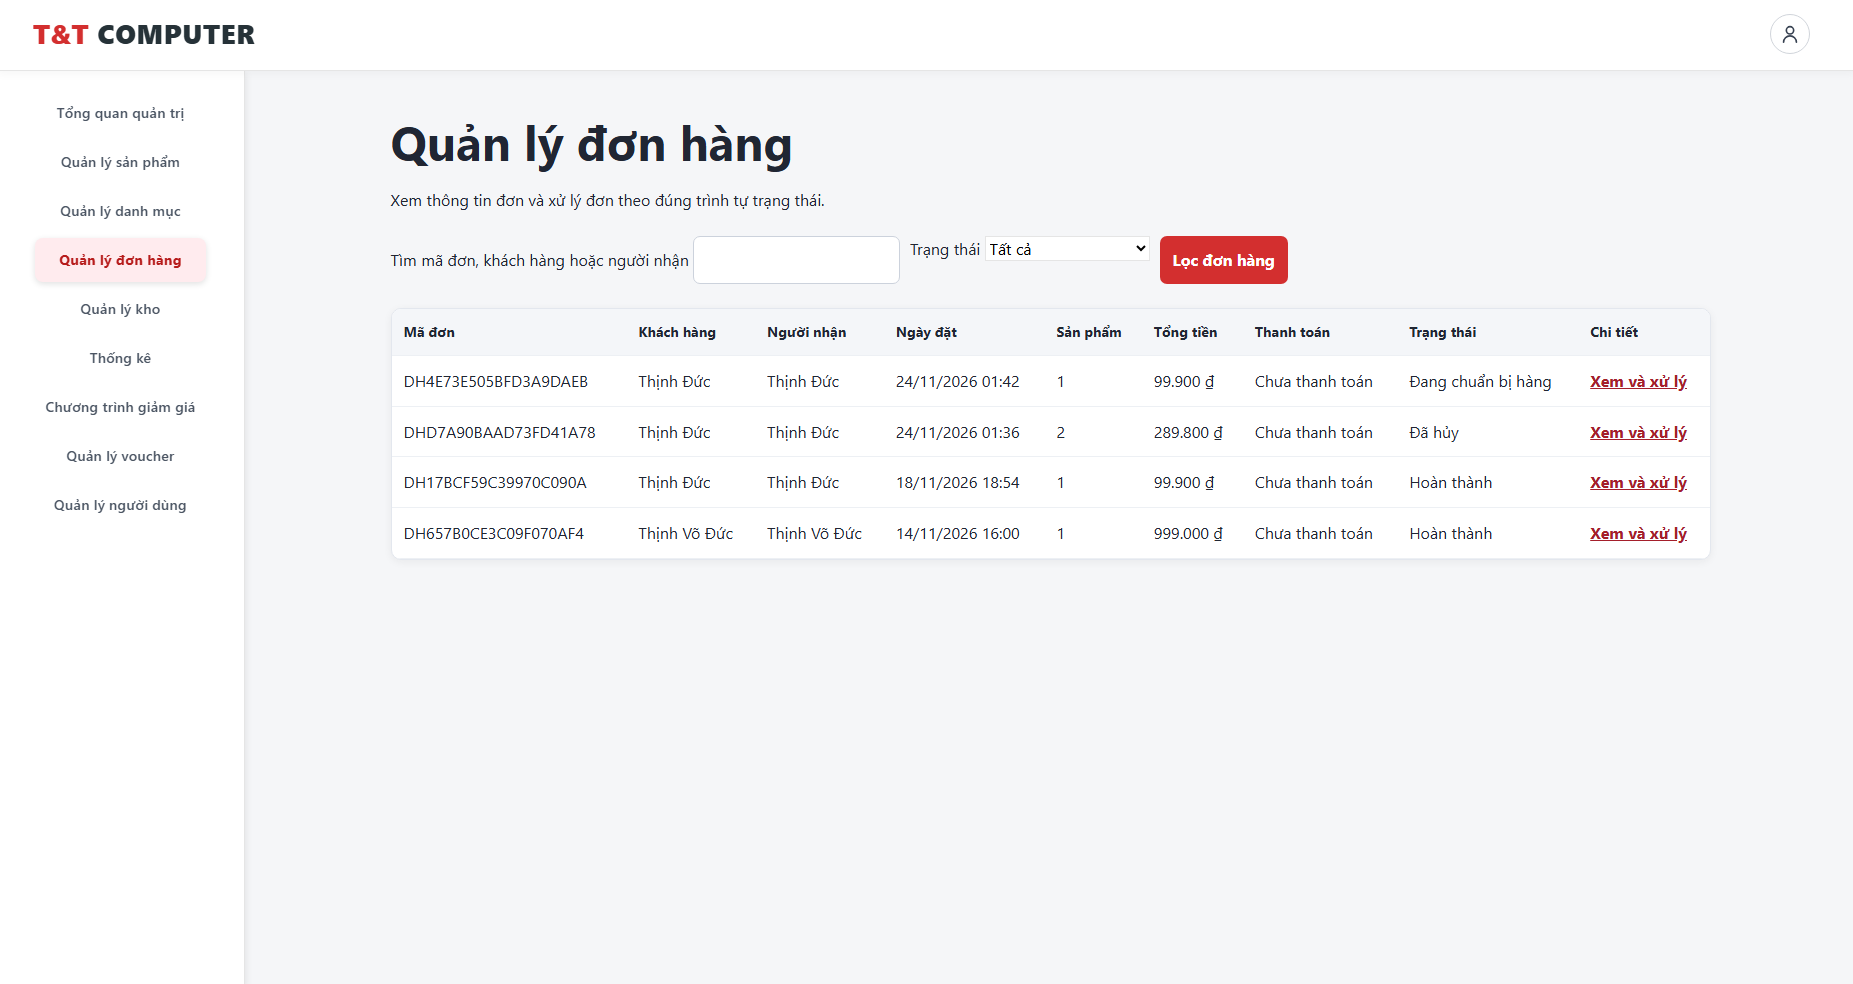
\includegraphics[width=0.95\textwidth,height=0.72\textheight,keepaspectratio]{TaiLieu/AnhChuong3/IMG24_admin_quan_ly_don_hang.png}
    \caption{Quản lý đơn hàng}
    \label{fig:img24-admin-don-hang}
\end{figure}
\begin{figure}[H]
    \centering
    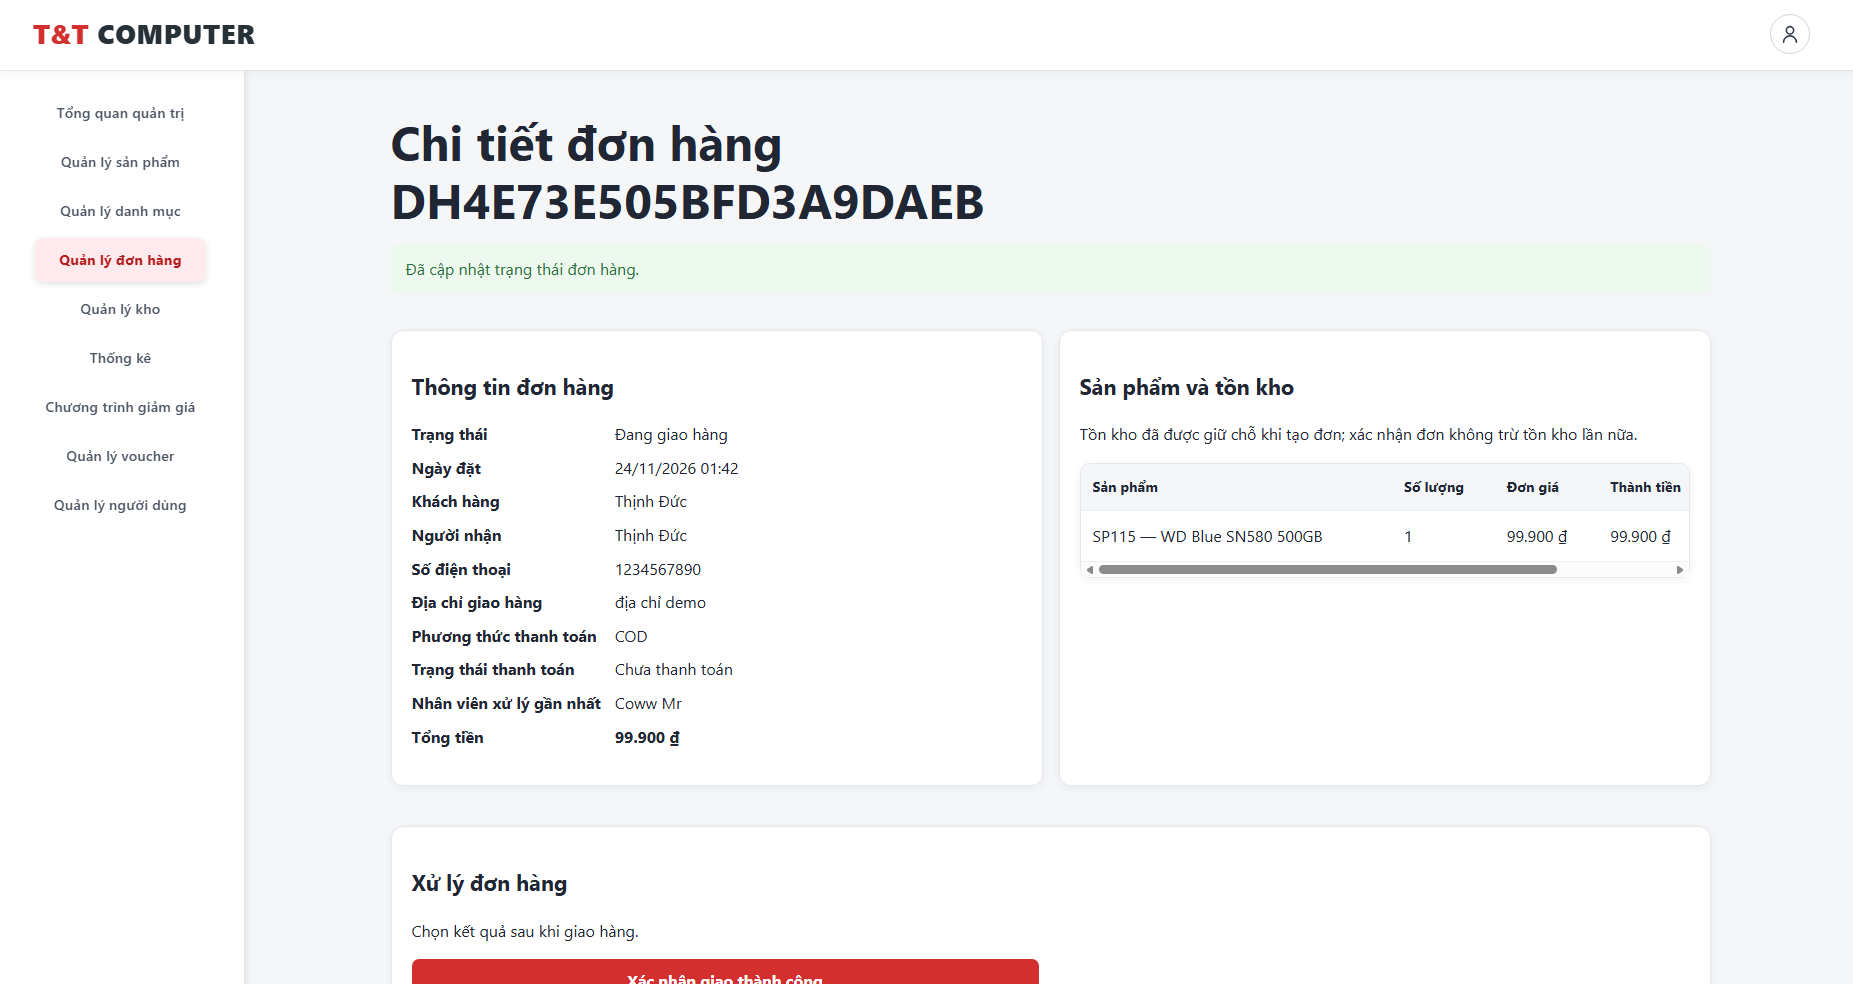
\includegraphics[width=0.95\textwidth,height=0.72\textheight,keepaspectratio]{TaiLieu/AnhChuong3/IMG25_admin_chi_tiet_cap_nhat_don.png}
    \caption{Chi tiết và thao tác xử lý đơn hàng của quản trị viên}
    \label{fig:img25-admin-chi-tiet-don}
\end{figure}
\begin{figure}[H]
    \centering
    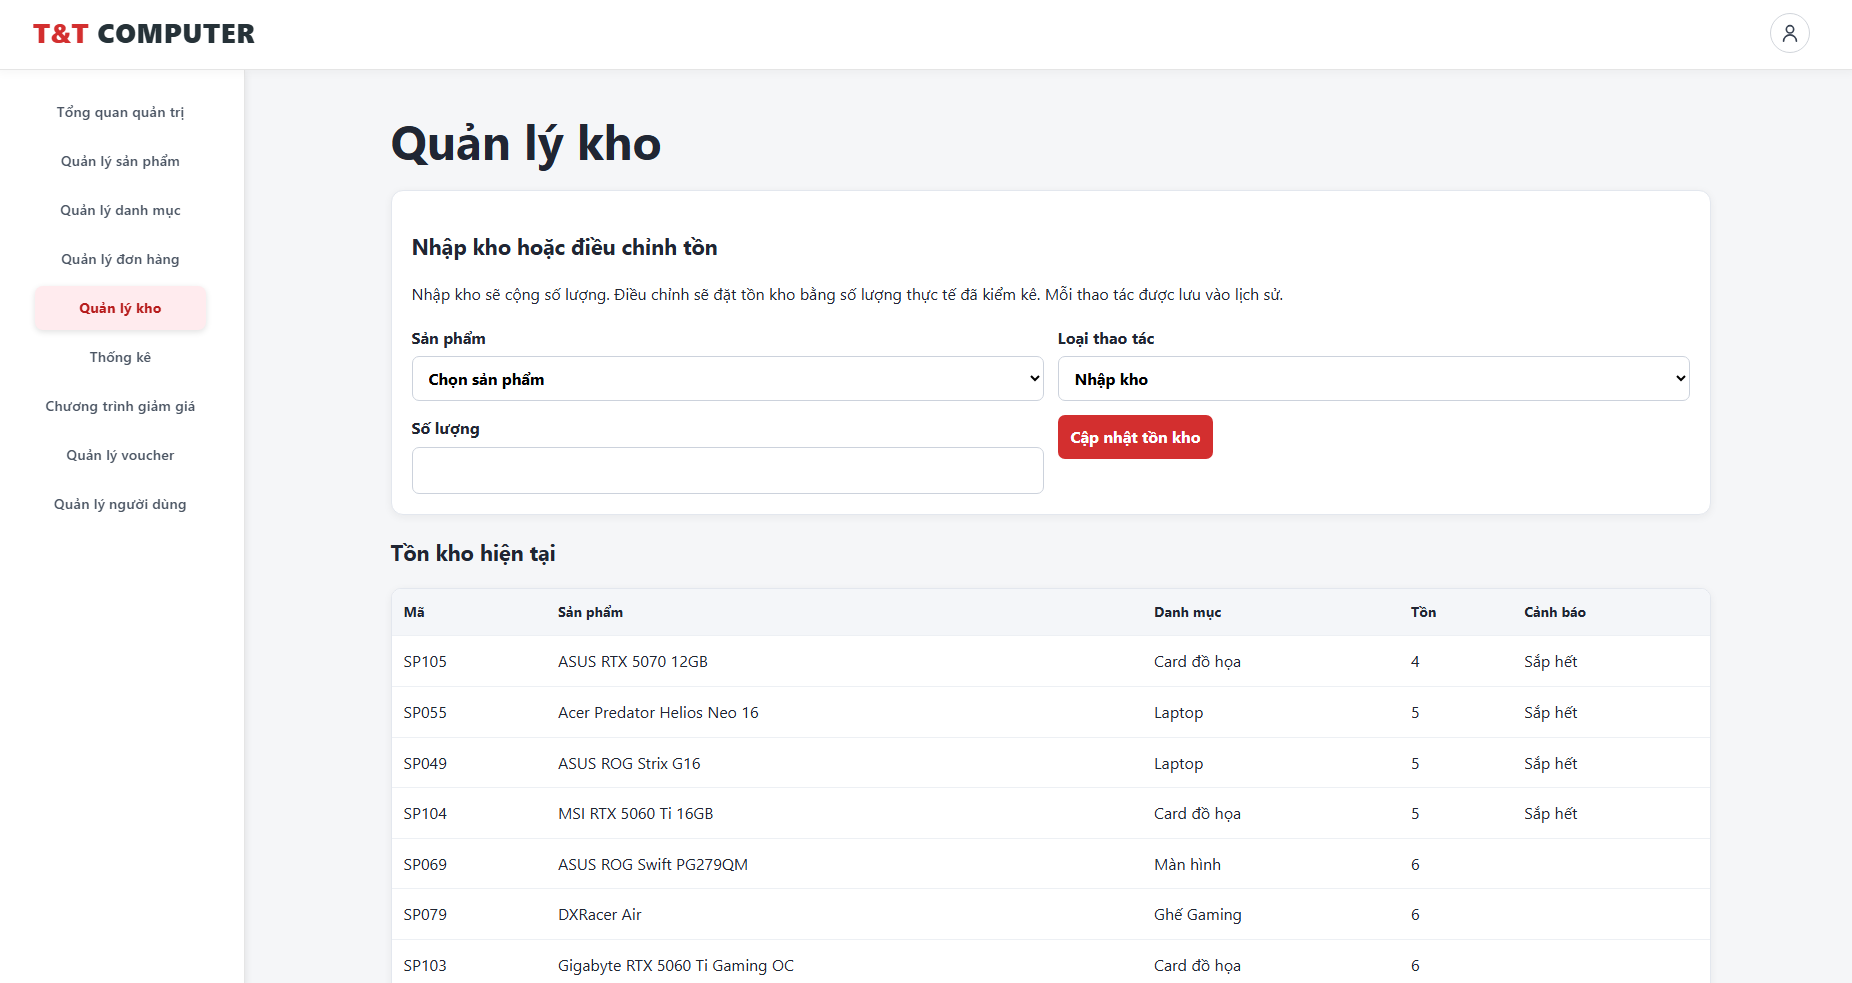
\includegraphics[width=0.95\textwidth,height=0.72\textheight,keepaspectratio]{TaiLieu/AnhChuong3/IMG26_admin_quan_ly_ton_kho.png}
    \caption{Quản lý tồn kho}
    \label{fig:img26-admin-ton-kho}
\end{figure}
\begin{figure}[H]
    \centering
    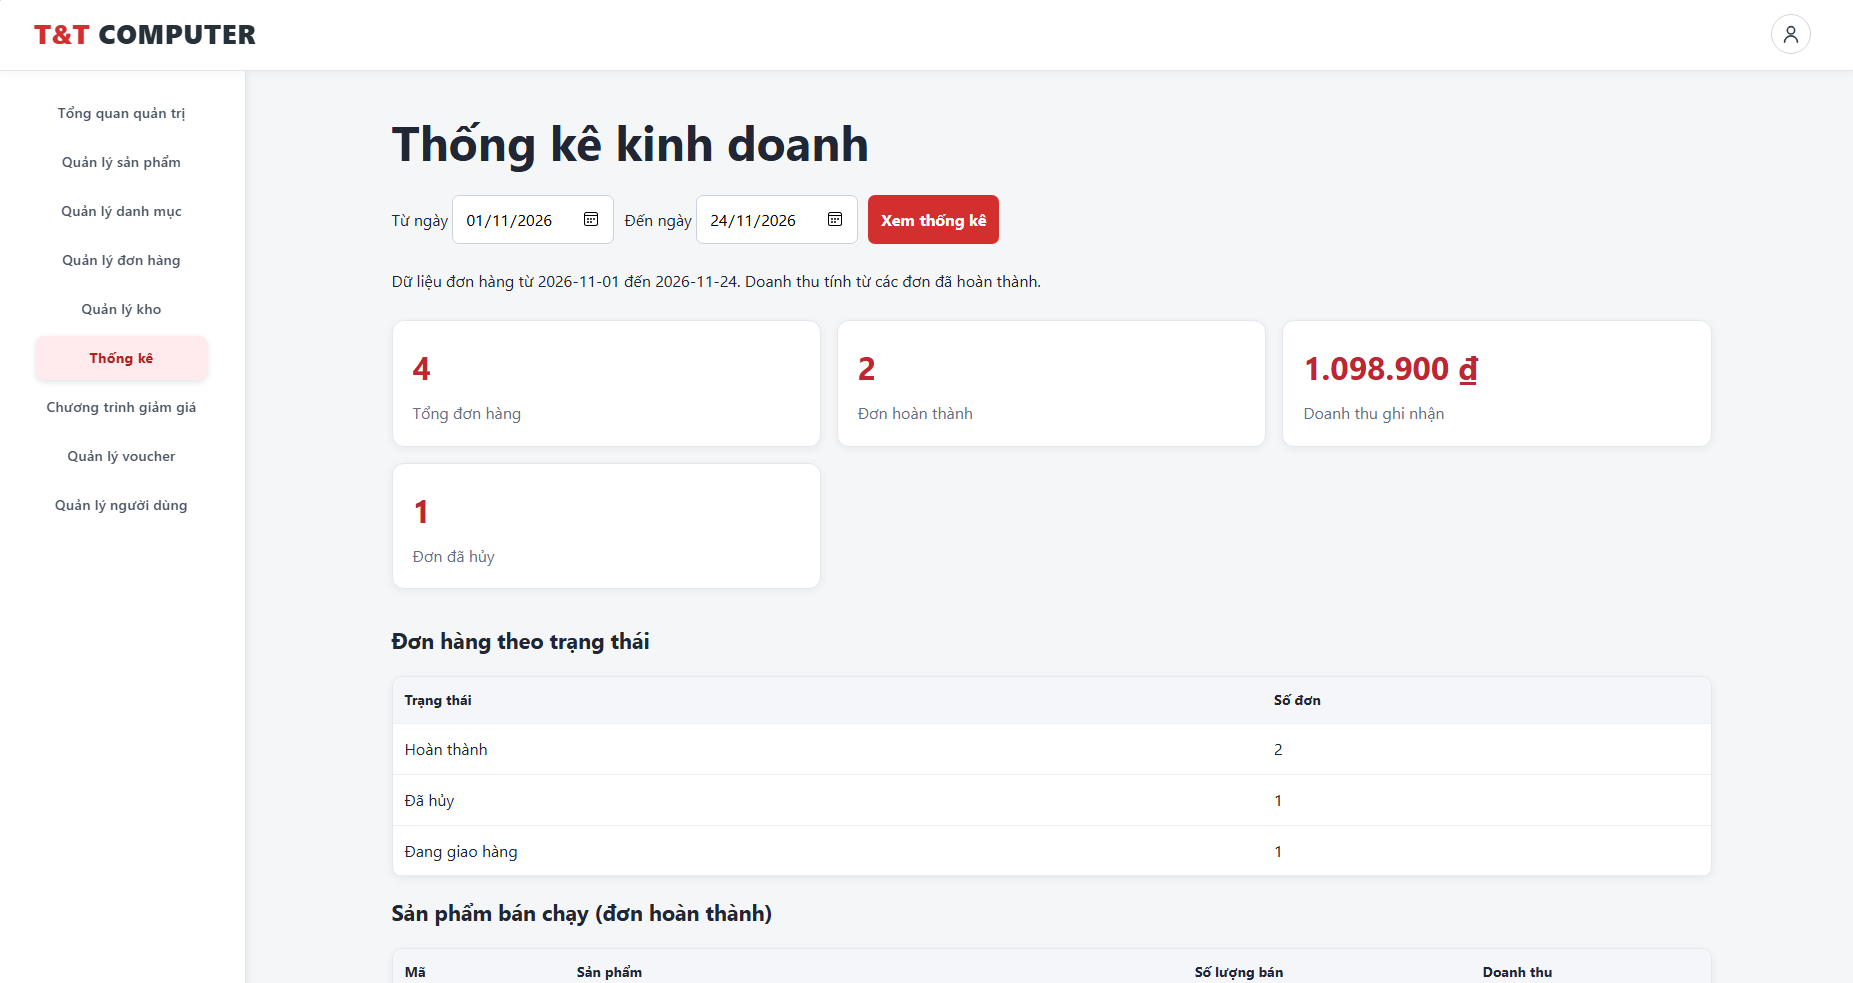
\includegraphics[width=0.95\textwidth,height=0.72\textheight,keepaspectratio]{TaiLieu/AnhChuong3/IMG27_admin_thong_ke.png}
    \caption{Thống kê quản trị}
    \label{fig:img27-admin-thong-ke}
\end{figure}
\begin{figure}[H]
    \centering
    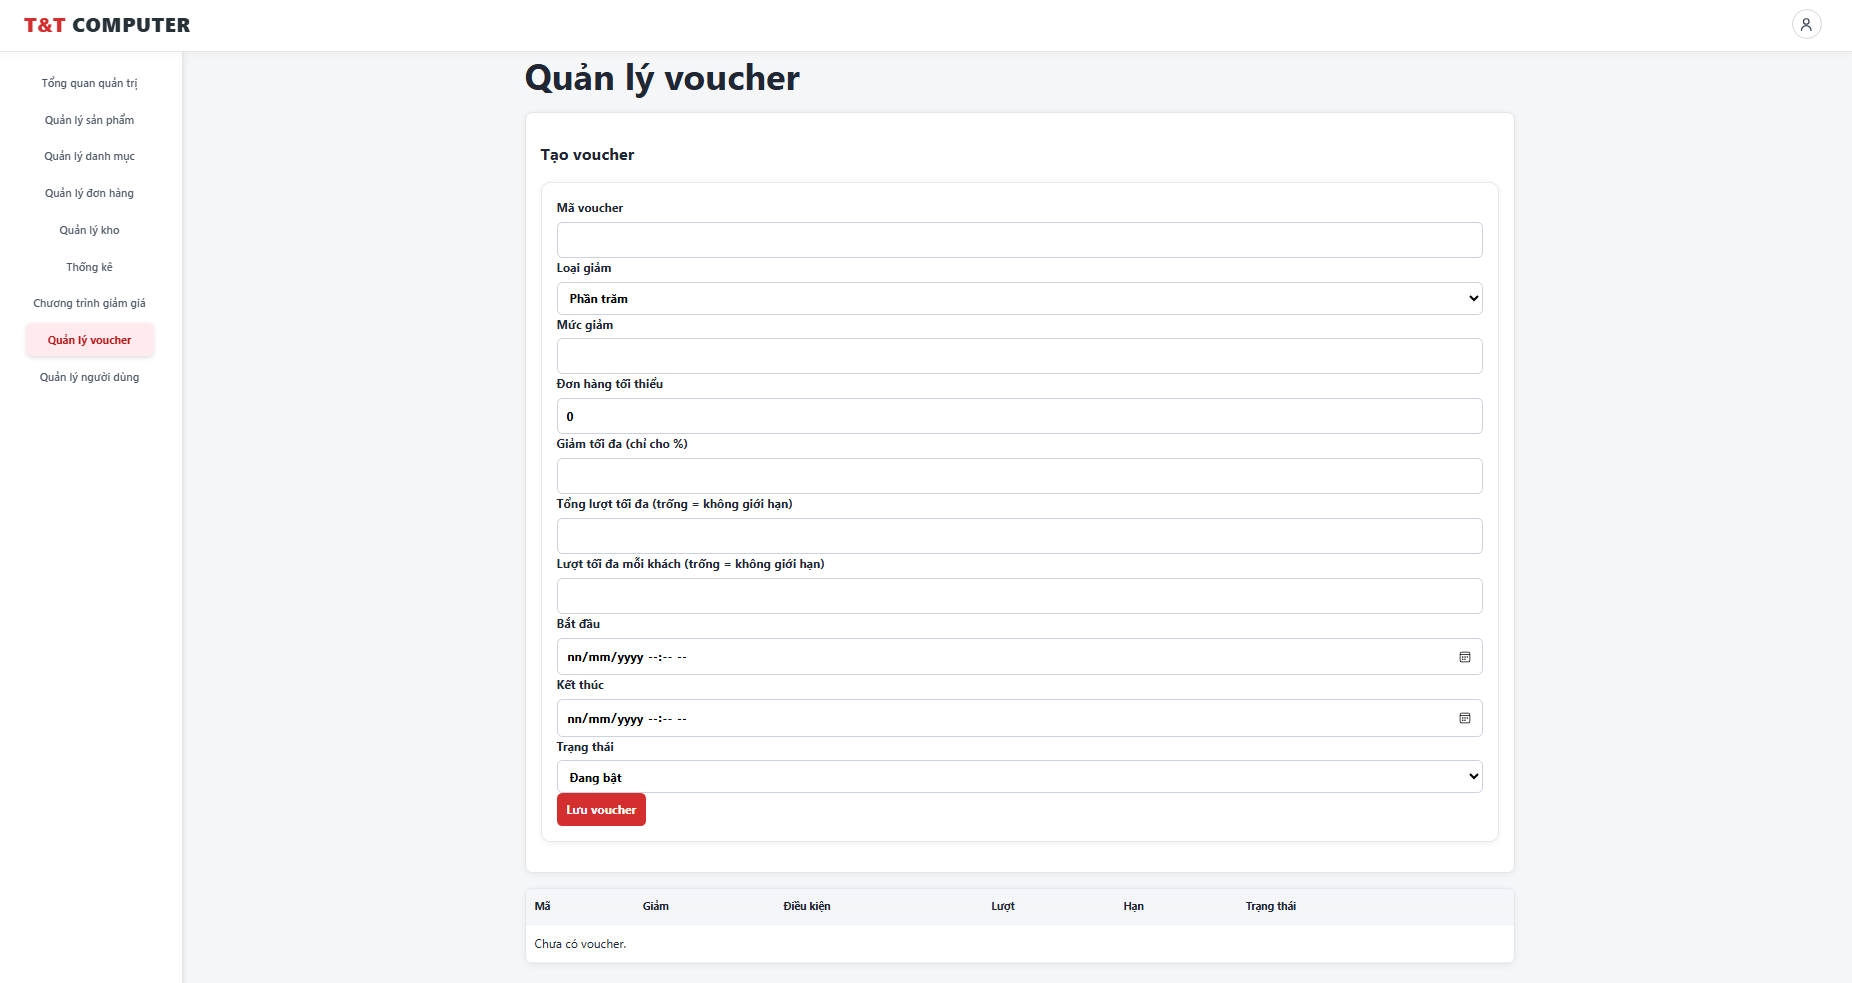
\includegraphics[width=0.95\textwidth,height=0.72\textheight,keepaspectratio]{TaiLieu/AnhChuong3/IMG28_admin_quan_ly_voucher.png}
    \caption{Quản lý voucher và khuyến mãi}
    \label{fig:img28-admin-voucher}
\end{figure}

\subsection{Tích hợp ngoài}
Luồng đăng nhập Google có trong mã nguồn và phụ thuộc cấu hình OAuth. Luồng SePay có khởi tạo checkout Sandbox, các URL trả về và endpoint IPN; controller kiểm tra chữ ký bí mật, trạng thái, loại giao dịch, tiền tệ và số tiền trước khi gọi model ghi nhận giao dịch. Bảng \texttt{GiaoDichThanhToan} lưu mã giao dịch cổng, số tiền, trạng thái và thời điểm. Những phần này là tích hợp được thể hiện trong source code; không có bằng chứng kiểm thử đầu-cuối trong tài liệu dự án.

\section{Minh họa quy trình nghiệp vụ}
Các sơ đồ tuần tự dưới đây mô tả luồng nghiệp vụ; các ảnh giao diện tiếp theo minh họa màn hình thực tế được cung cấp cho báo cáo. Ảnh giao diện không thay thế nhật ký hoặc biên bản kiểm thử.

\subsection{Tra cứu sản phẩm}
\begin{figure}[H]
    \centering
    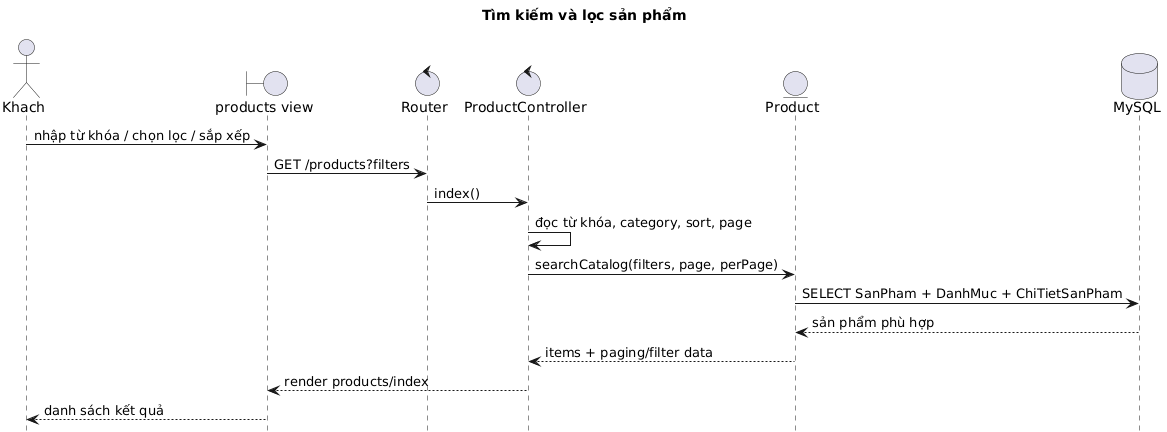
\includegraphics[width=0.98\textwidth,keepaspectratio]{Chapter_3/Images_sequence/TrinhTuUC03.png}
    \caption{Sơ đồ tuần tự tra cứu sản phẩm (UC03)}
    \label{fig:chap3-uc03}
\end{figure}

\subsection{Đặt hàng và chọn phương thức thanh toán}
\begin{figure}[H]
    \centering
    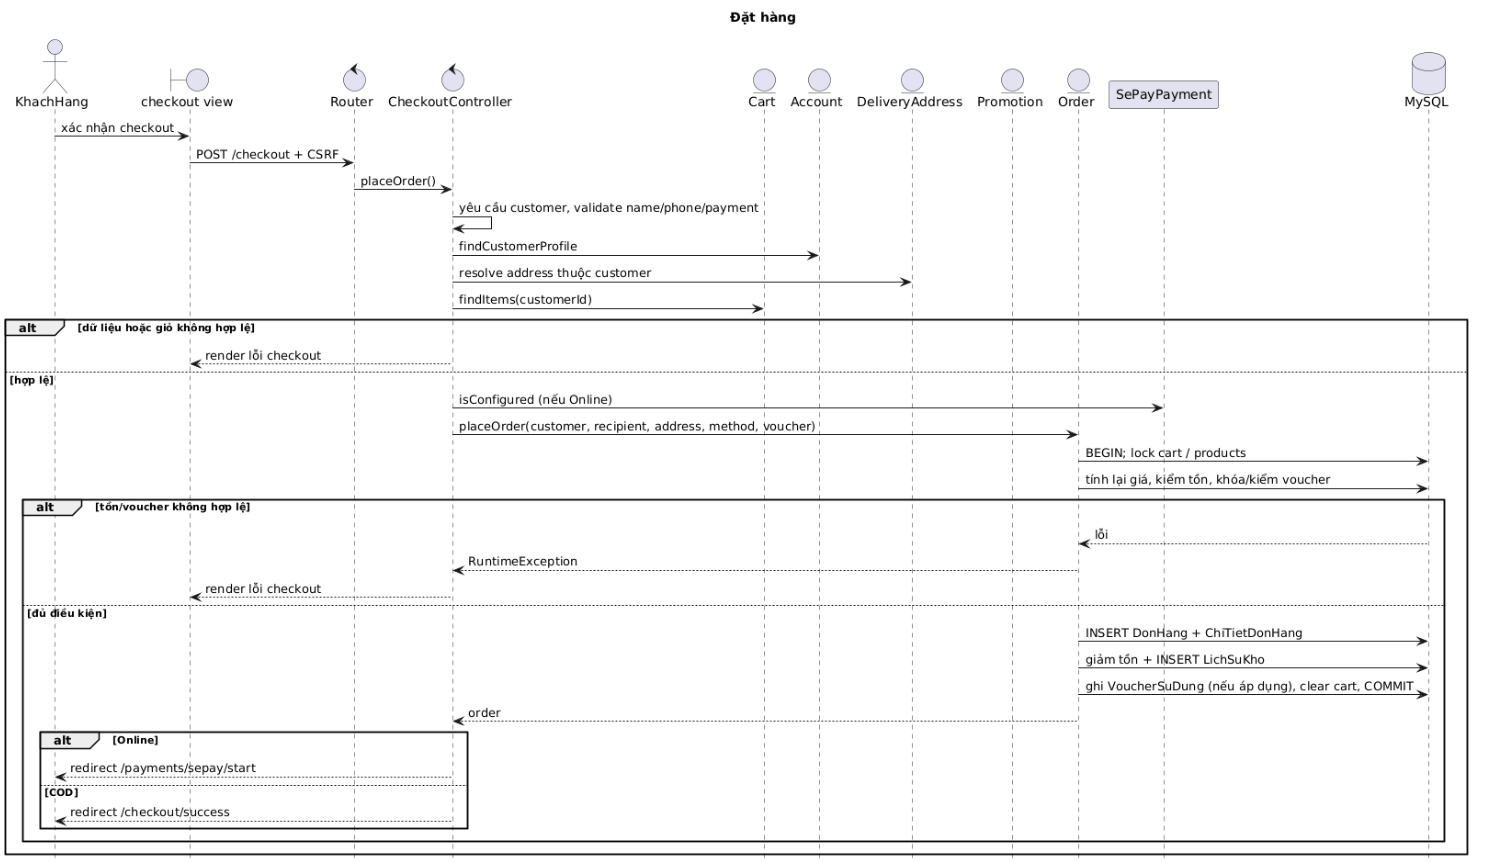
\includegraphics[width=0.98\textwidth,keepaspectratio]{Chapter_3/Images_sequence/TrinhTuUC05.png}
    \caption{Sơ đồ tuần tự tạo đơn, kiểm tra voucher và tồn kho (UC05)}
    \label{fig:chap3-uc05}
\end{figure}
Sơ đồ cho thấy đơn, chi tiết đơn, thay đổi tồn và lượt dùng voucher được xử lý khi tạo đơn. Đơn COD đi tới trang xác nhận; đơn Online mới chuyển sang checkout SePay. Việc khách được đưa về trang kết quả của cổng không thay thế việc xác minh IPN.

\begin{figure}[H]
    \centering
    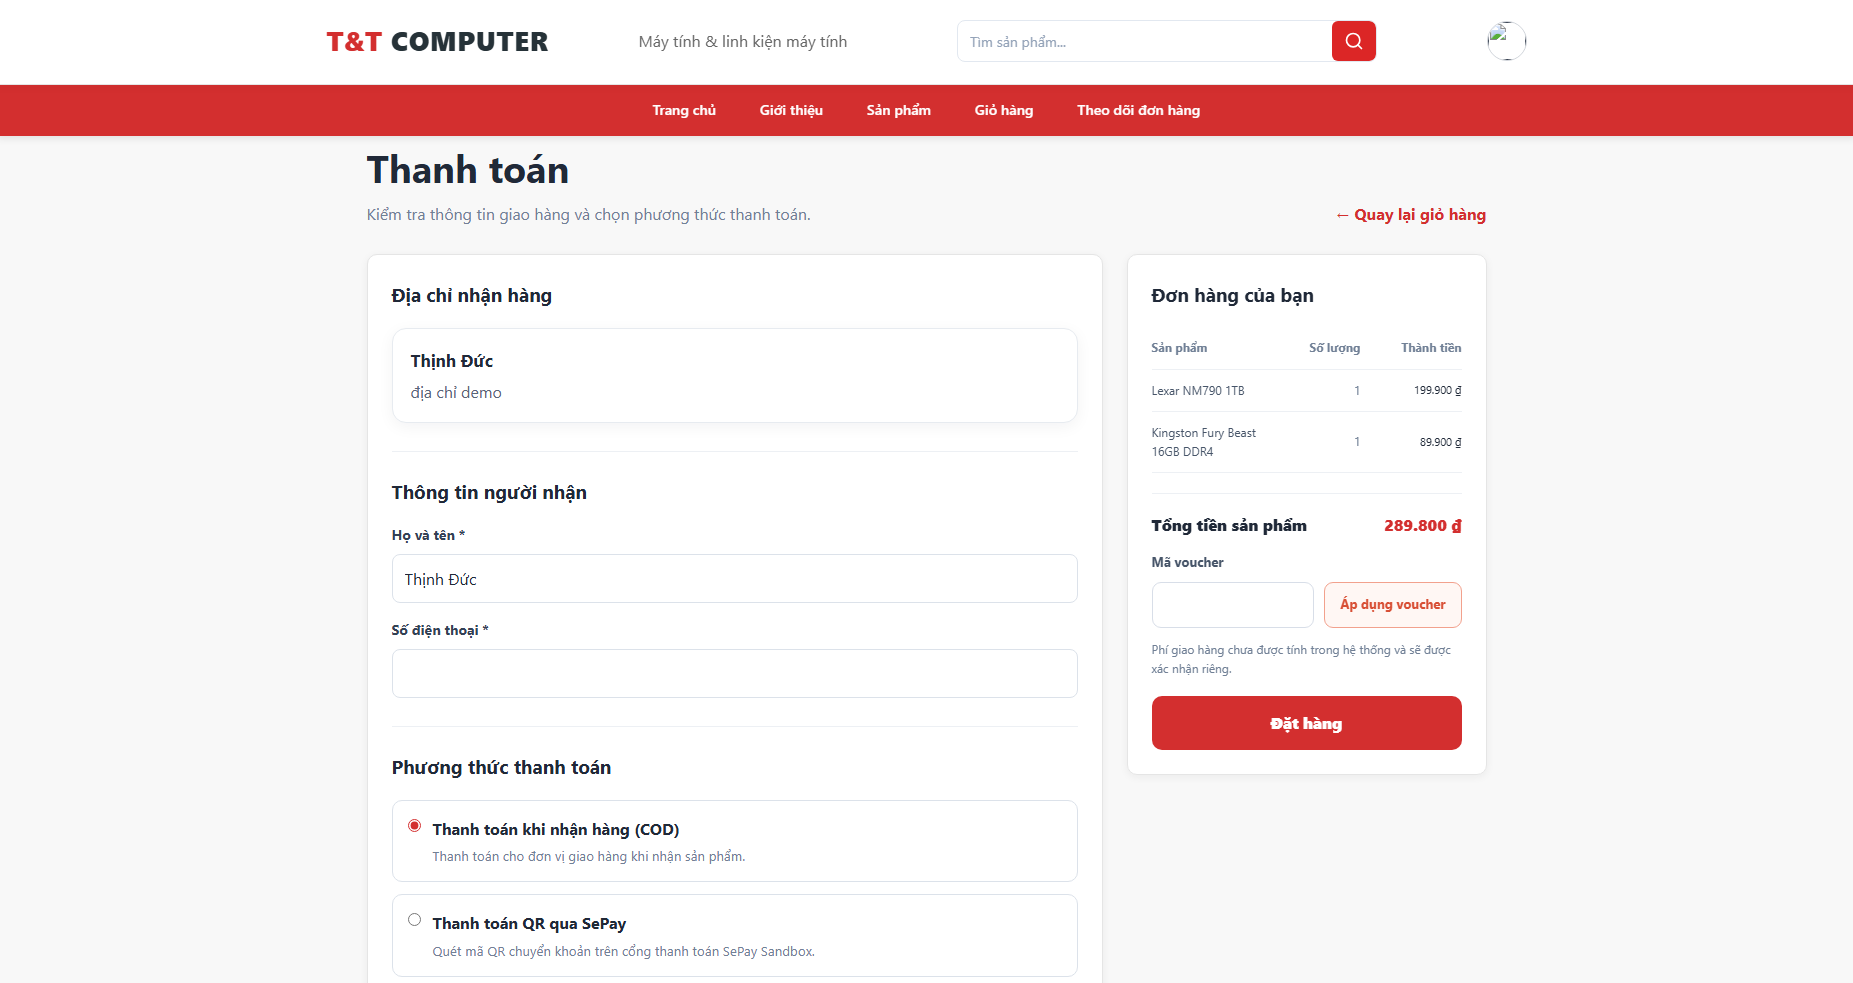
\includegraphics[width=0.95\textwidth,height=0.72\textheight,keepaspectratio]{TaiLieu/AnhChuong3/IMG09_checkout_thong_tin_giao_hang_IMG10_checkout_chon_cod.png}
    \caption{Màn hình checkout với thông tin giao hàng và lựa chọn COD}
    \label{fig:img09-checkout-cod}
\end{figure}
\begin{figure}[H]
    \centering
    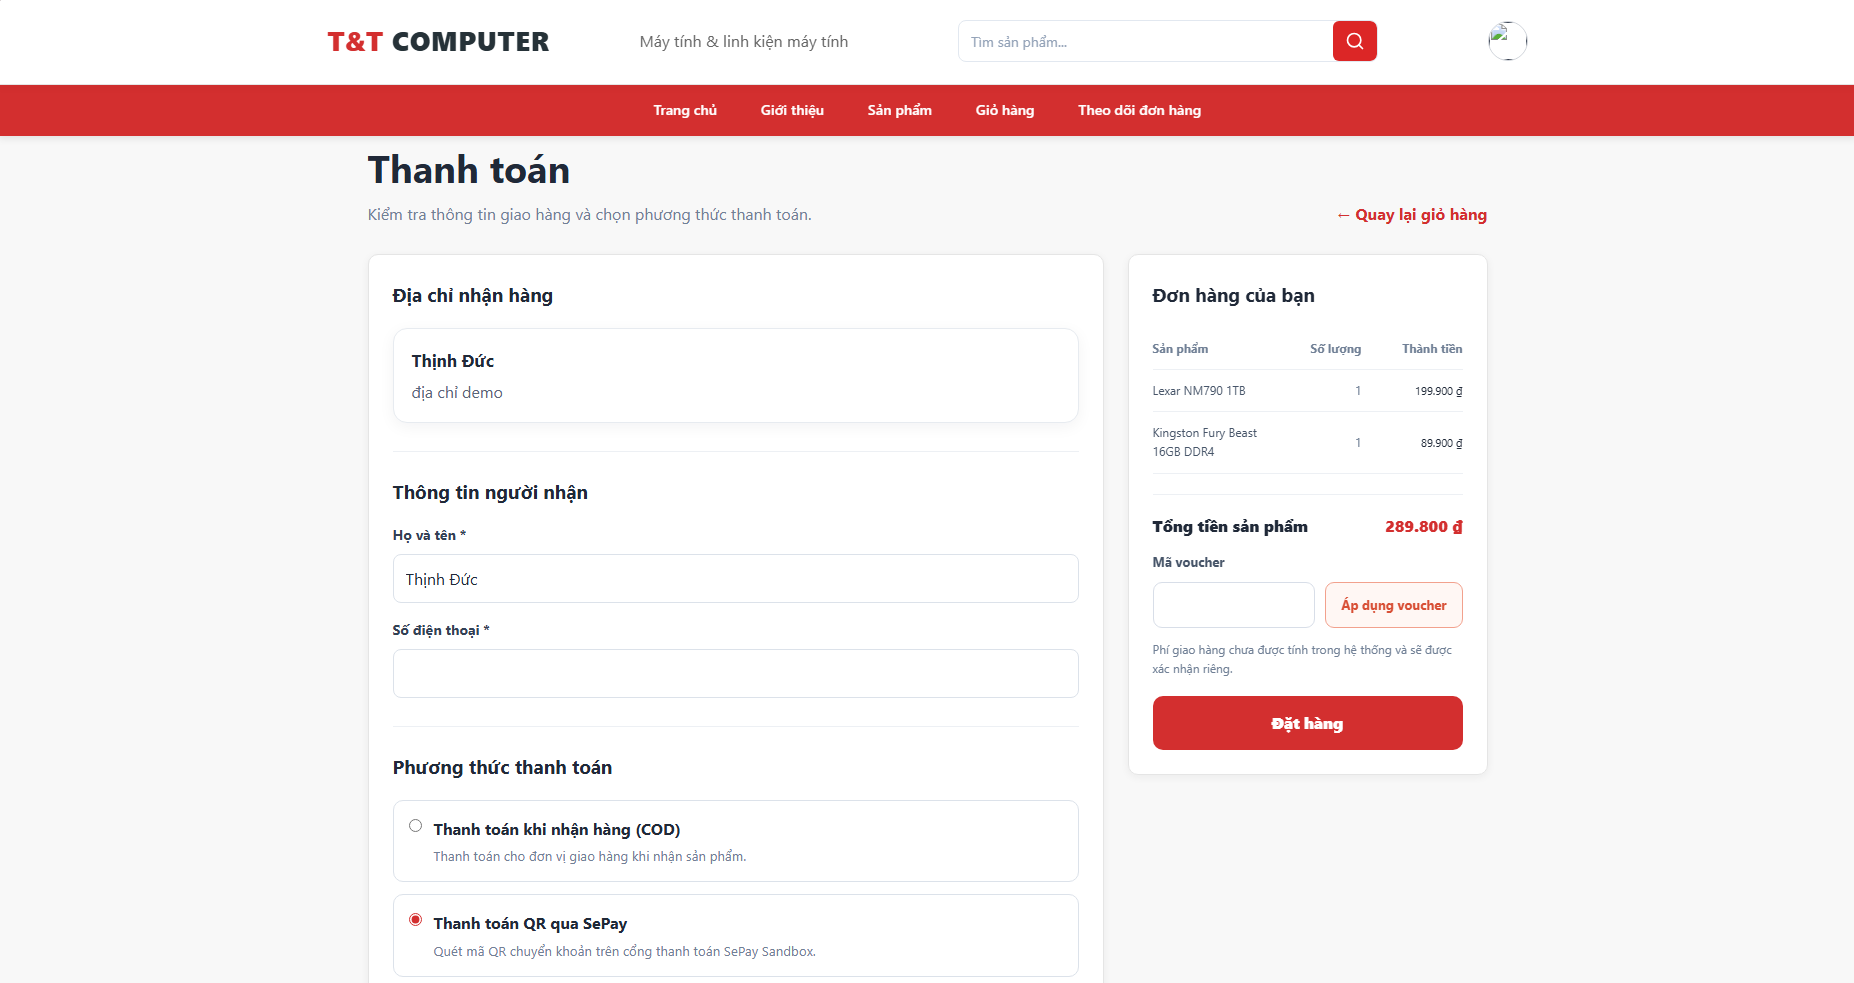
\includegraphics[width=0.95\textwidth,height=0.72\textheight,keepaspectratio]{TaiLieu/AnhChuong3/IMG11_checkout_chon_sepay_sandbox.png}
    \caption{Lựa chọn thanh toán SePay Sandbox tại checkout}
    \label{fig:img11-checkout-sepay}
\end{figure}
\begin{figure}[H]
    \centering
    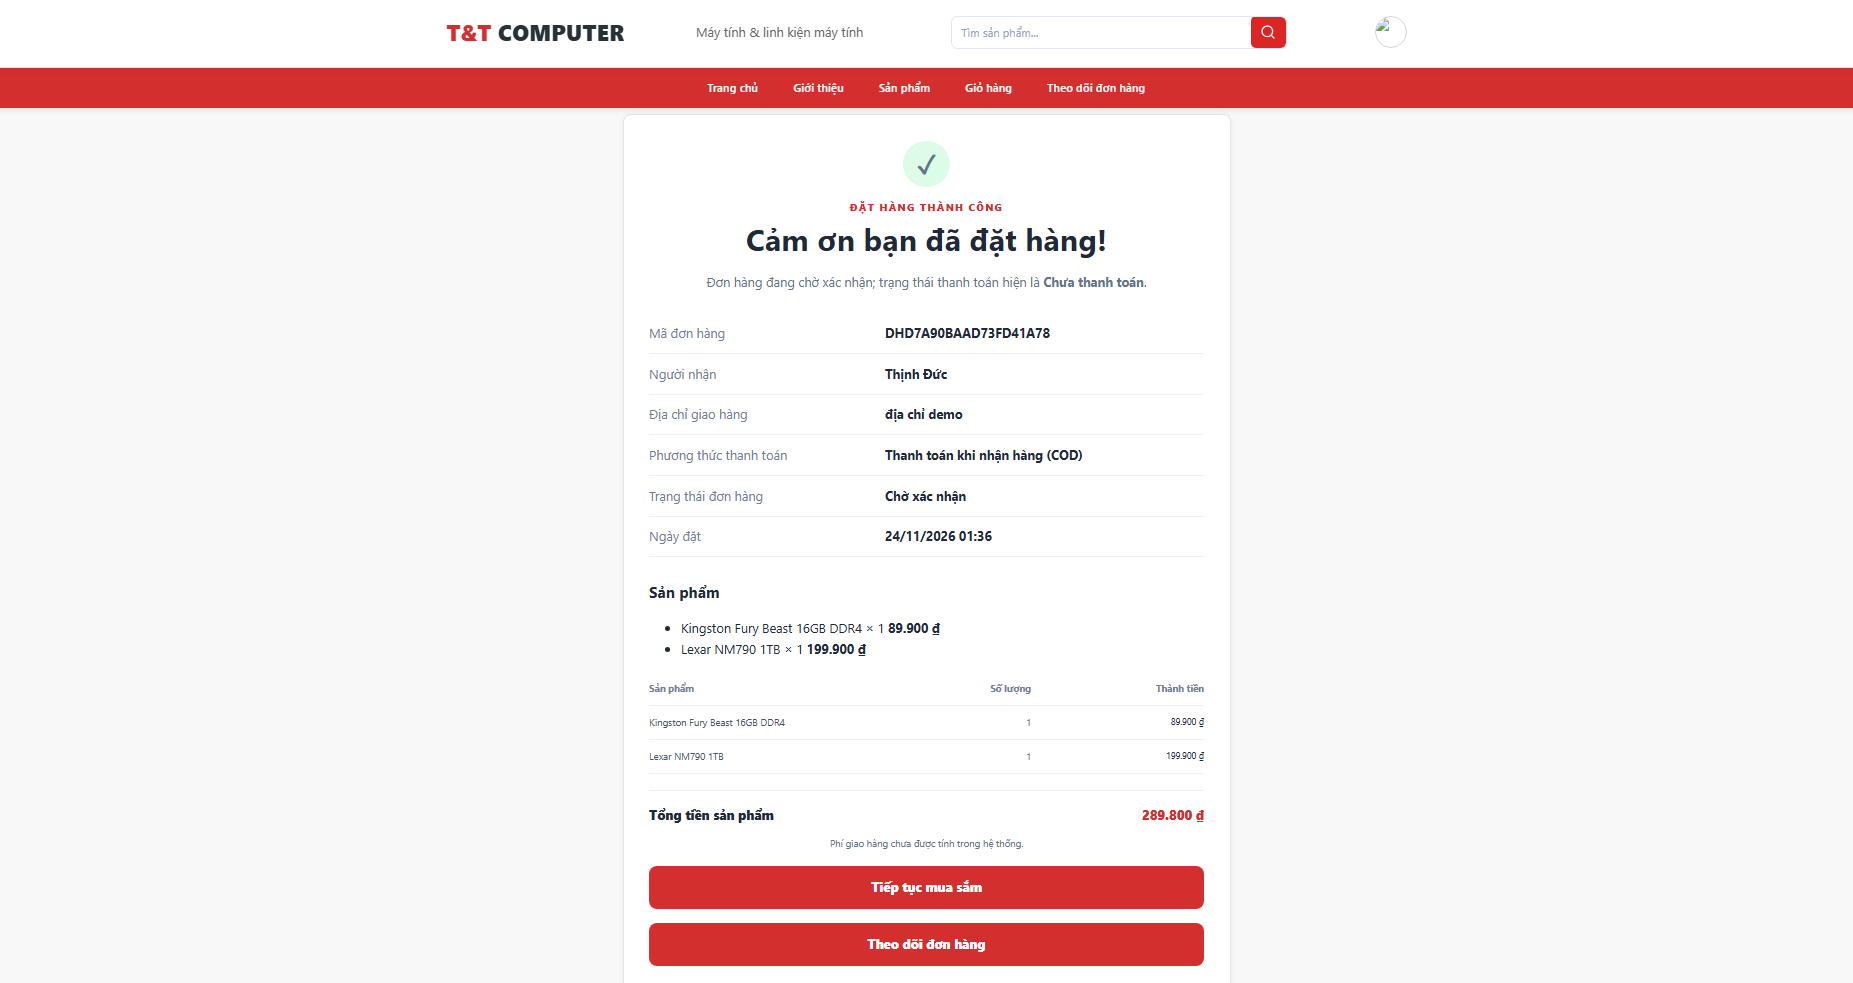
\includegraphics[width=0.95\textwidth,height=0.72\textheight,keepaspectratio]{TaiLieu/AnhChuong3/IMG12_dat_hang_thanh_cong_cod.png}
    \caption{Trang xác nhận tạo đơn COD; đơn vẫn ở trạng thái chưa thanh toán}
    \label{fig:img12-ket-qua-cod}
\end{figure}

\subsection{Theo dõi và hủy đơn}
\begin{figure}[H]
    \centering
    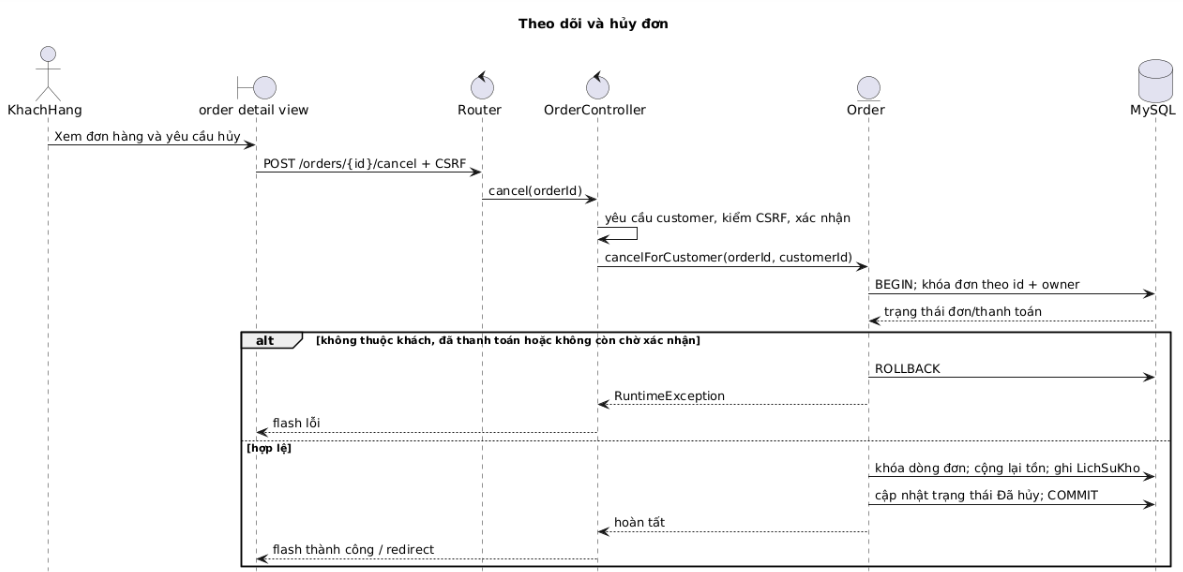
\includegraphics[width=0.98\textwidth,keepaspectratio]{Chapter_3/Images_sequence/TrinhTuUC07.png}
    \caption{Sơ đồ tuần tự theo dõi và yêu cầu hủy đơn (UC07)}
    \label{fig:chap3-uc07}
\end{figure}
Trong mã nguồn, khách chỉ hủy được đơn chưa thanh toán còn ở trạng thái Chờ xác nhận; thao tác hoàn lại tồn và ghi lịch sử kho nằm trong transaction. Không có nhánh tự hủy theo thời hạn được triển khai.

\begin{figure}[H]
    \centering
    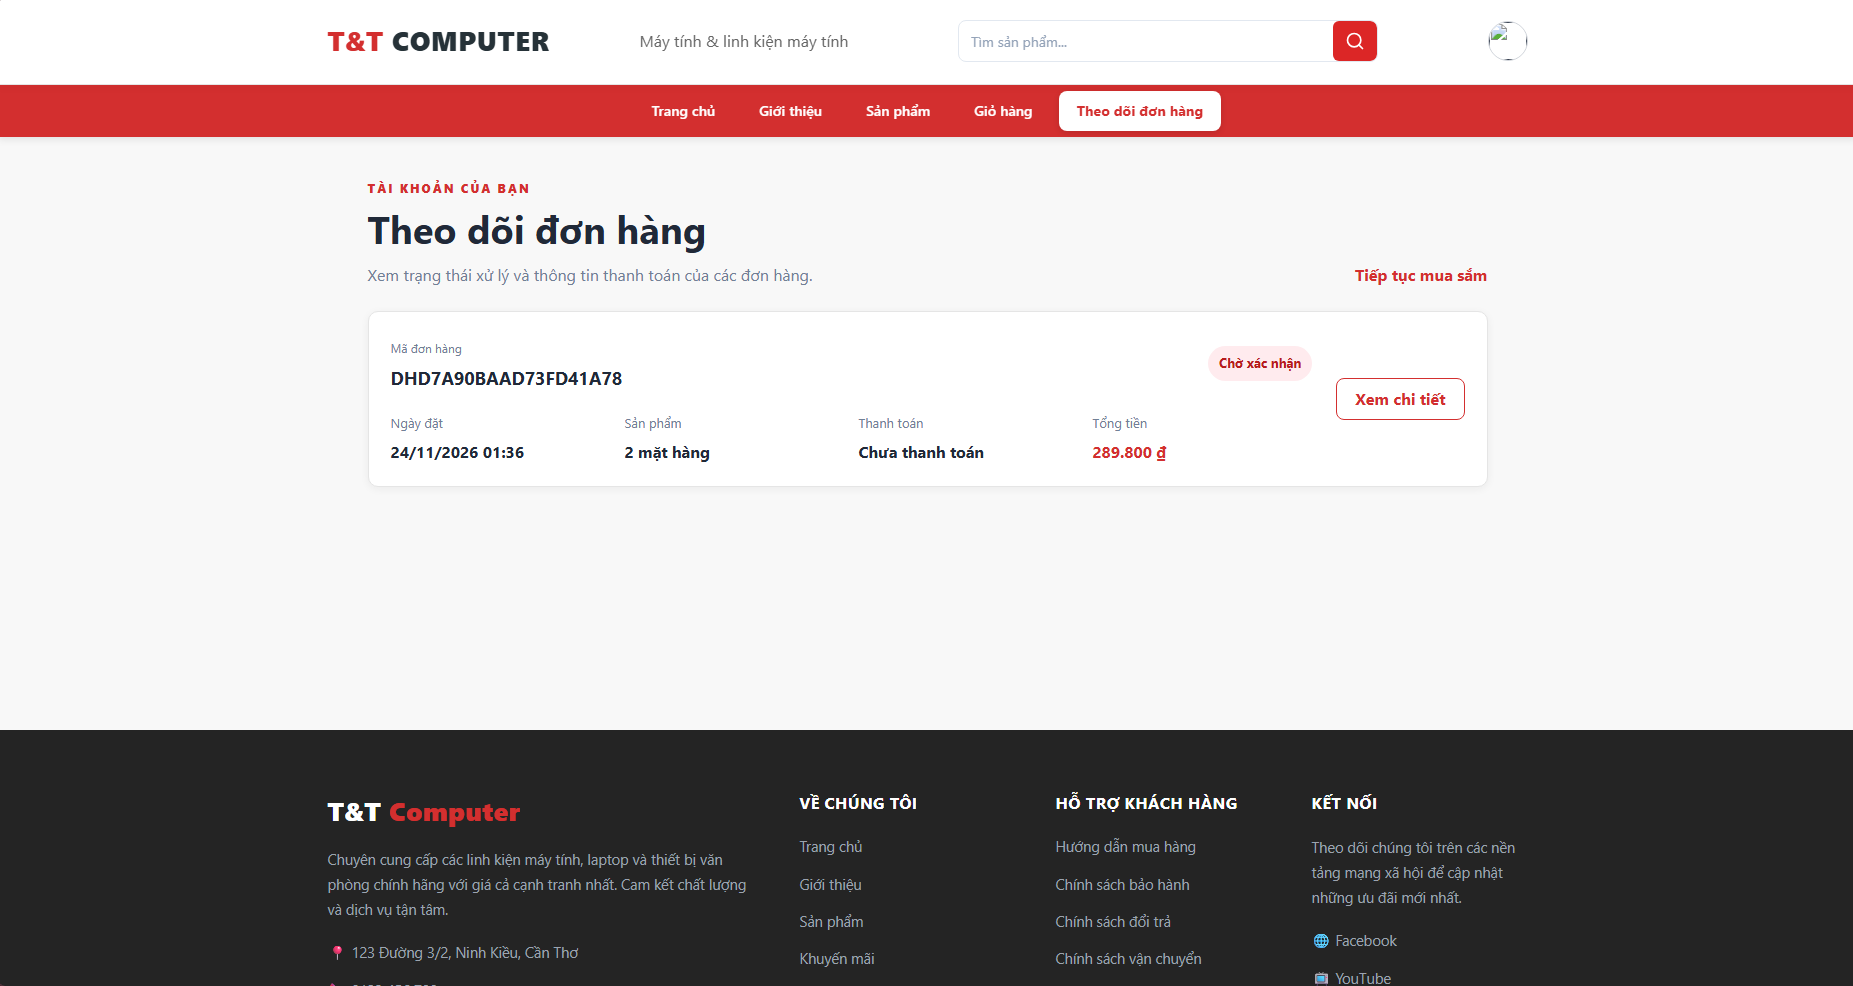
\includegraphics[width=0.95\textwidth,height=0.72\textheight,keepaspectratio]{TaiLieu/AnhChuong3/IMG13_lich_su_don_hang.png}
    \caption{Lịch sử đơn hàng của khách hàng}
    \label{fig:img13-lich-su-don}
\end{figure}
\begin{figure}[H]
    \centering
    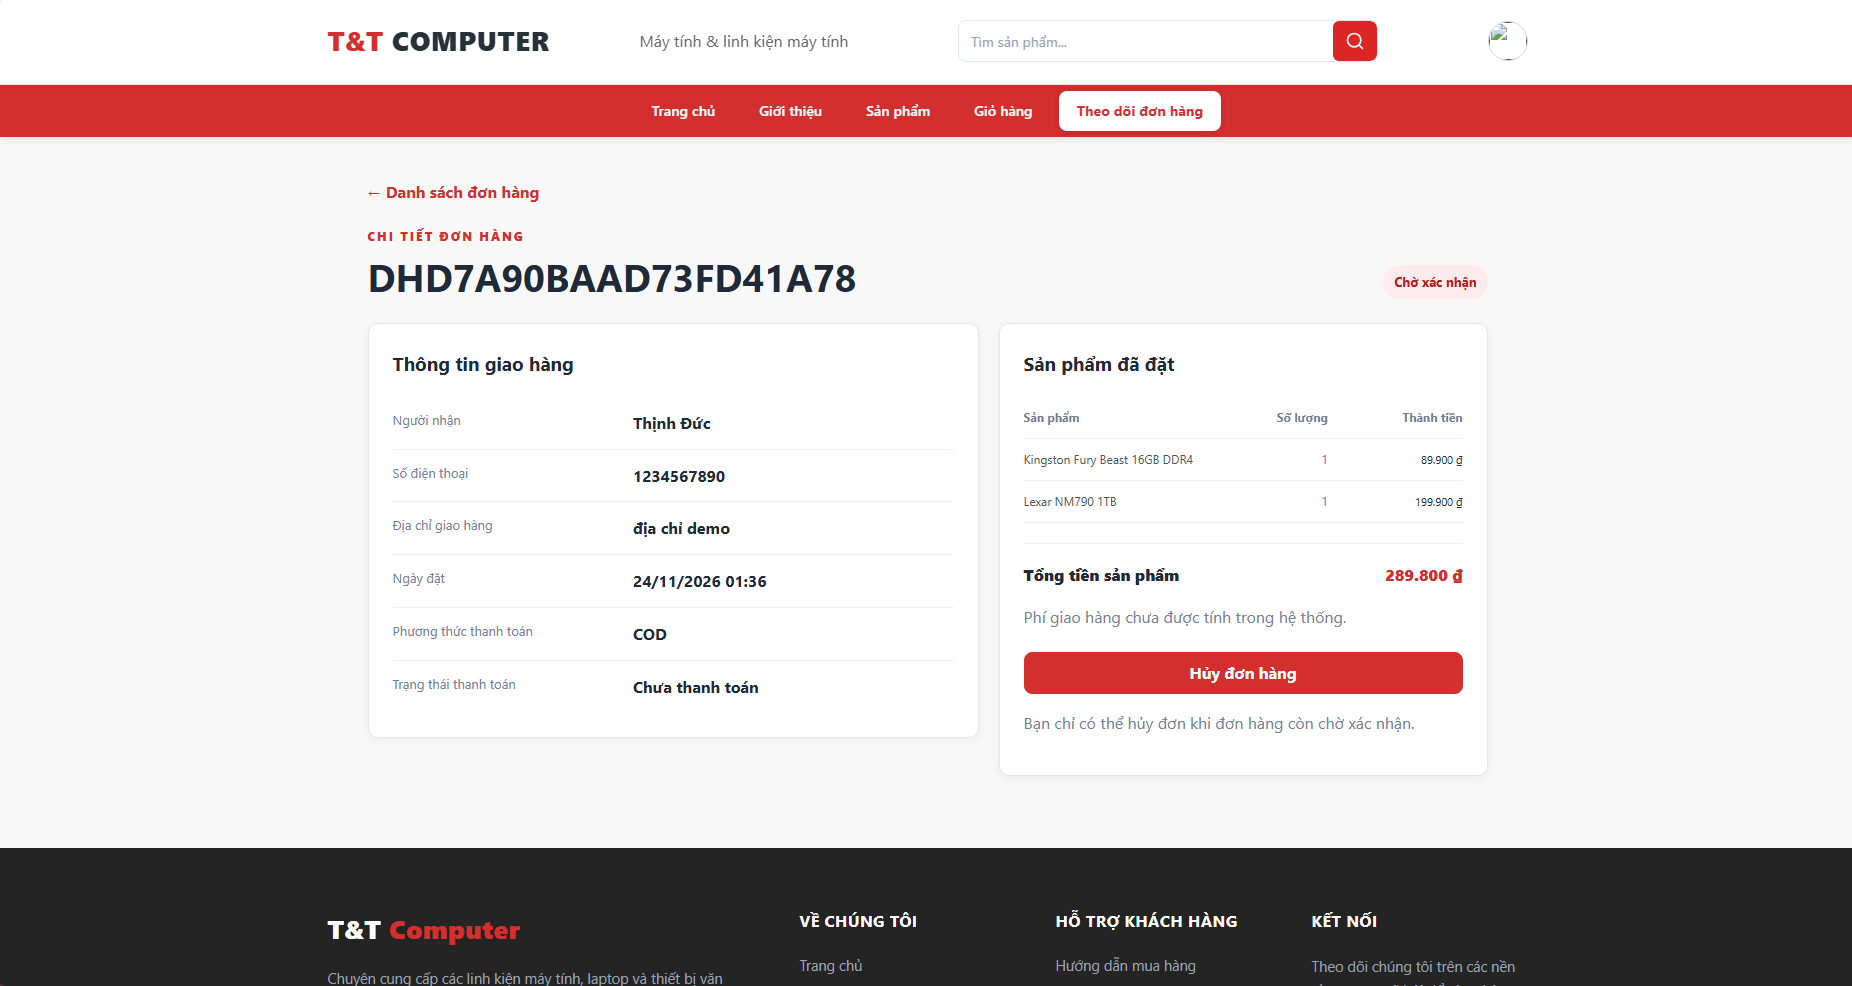
\includegraphics[width=0.95\textwidth,height=0.72\textheight,keepaspectratio]{TaiLieu/AnhChuong3/IMG14_chi_tiet_theo_doi_don_hang.png}
    \caption{Chi tiết và trạng thái đơn hàng}
    \label{fig:img14-chi-tiet-don}
\end{figure}
\begin{figure}[H]
    \centering
    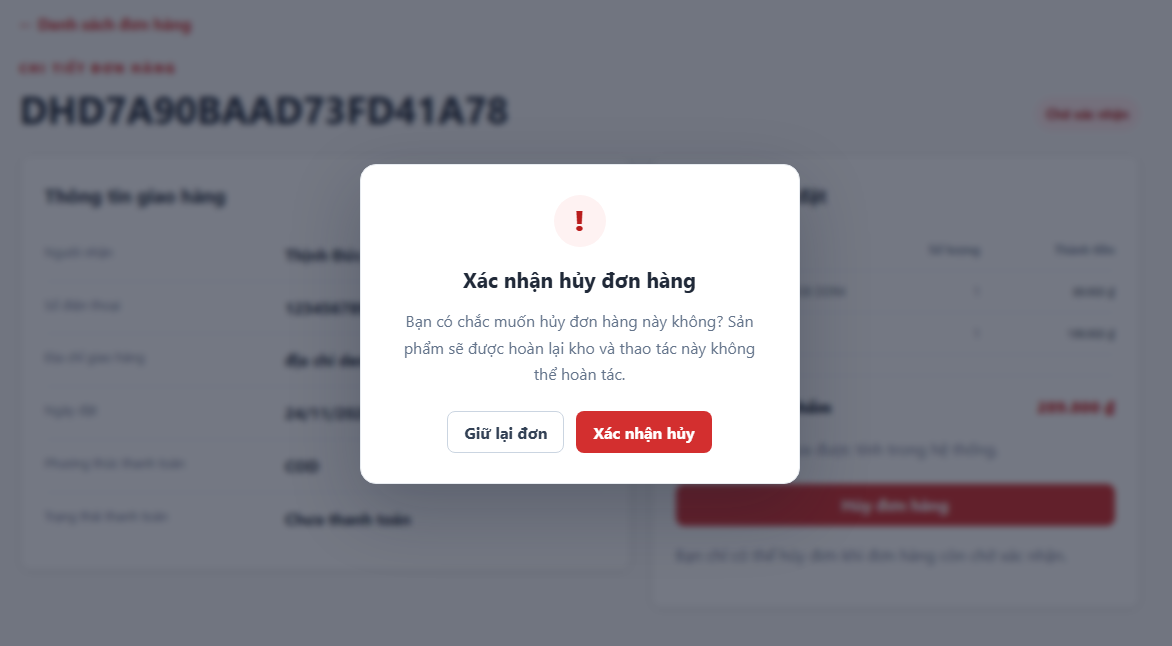
\includegraphics[width=0.95\textwidth,height=0.72\textheight,keepaspectratio]{TaiLieu/AnhChuong3/IMG15_huy_don_chua_thanh_toan_01.png}
    \caption{Hộp thoại xác nhận hủy đơn hàng chưa thanh toán}
    \label{fig:img15-xac-nhan-huy}
\end{figure}
\begin{figure}[H]
    \centering
    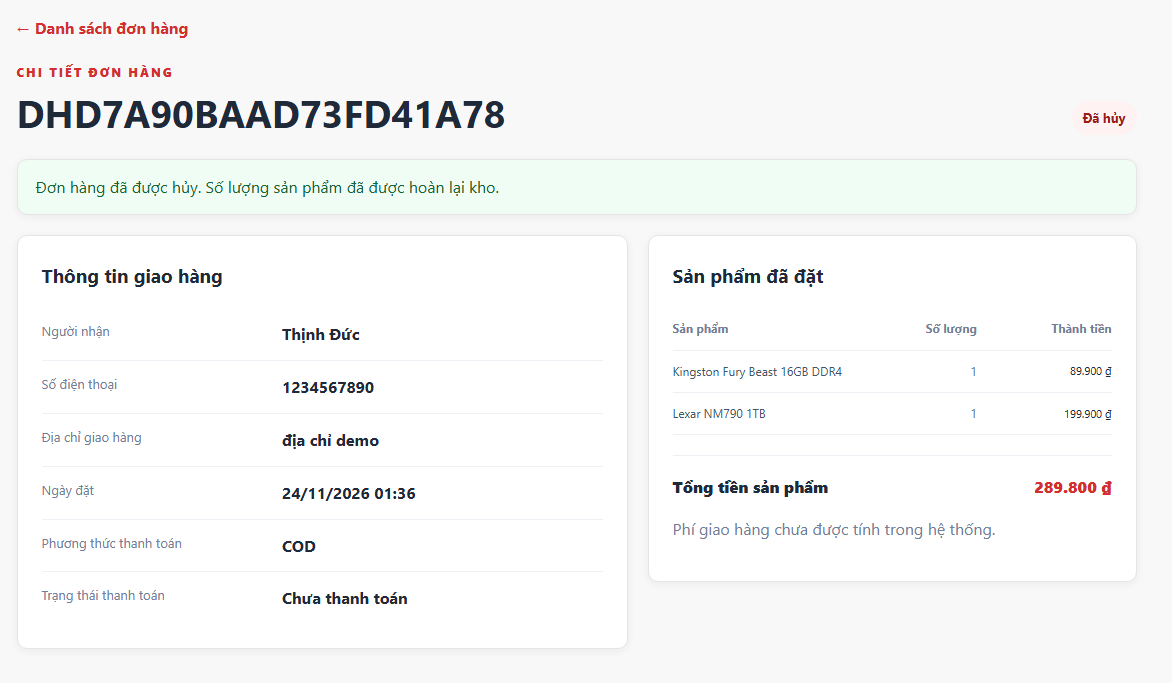
\includegraphics[width=0.95\textwidth,height=0.72\textheight,keepaspectratio]{TaiLieu/AnhChuong3/IMG15_huy_don_chua_thanh_toan_02.png}
    \caption{Thông báo đơn hàng đã hủy và số lượng được hoàn lại kho}
    \label{fig:img15-ket-qua-huy}
\end{figure}

\section{Đánh giá và thảo luận}
Đối chiếu source cho thấy các luồng cốt lõi về tài khoản, danh mục sản phẩm, giỏ hàng, tạo đơn, quản trị và cập nhật tồn kho đã có thành phần xử lý tương ứng. Một số nghiệp vụ có transaction và kiểm tra dữ liệu tại máy chủ, giúp giữ nhất quán dữ liệu khi thao tác thất bại. Đây là đánh giá dựa trên mã nguồn, chưa phải kết luận từ nghiệm thu vận hành.

Các phần mới triển khai một phần hoặc chưa có bằng chứng gồm: bước ghi nhận đã thu tiền COD; vận hành thanh toán SePay ngoài Sandbox; tác vụ nền tự hủy đơn quá hạn; và kiểm thử động có biên bản cho các nhánh nghiệp vụ. Ảnh chụp giao diện được dùng để minh họa các màn hình, nhưng không chứng minh tích hợp SePay đầu-cuối hay kết quả kiểm thử đầy đủ. Chương 4 trình bày các hạn chế và hướng hoàn thiện.
